% I seguenti commenti speciali impostano:
% 1. 
% 2. PDFLaTeX come motore di composizione;
% 3. tesi.tex come documento principale;
% 4. il controllo ortografico italiano per l'editor.

% !TEX encoding = UTF-8
% !TEX TS-program = pdflatex
% !TEX root = Lahmer_Abdelilah_tesi.tex
% !TEX spellcheck = it-IT

\documentclass[11pt,                    % corpo del font principale
               a4paper,                 % carta A4
               twoside,                 % impagina per fronte-retro
               openright,               % inizio capitoli a destra
               english,                 
               italian,                 
               ]{book}    

\usepackage[utf8]{inputenc}             % codifica di input; anche [latin1] va bene
                                        % NOTA BENE! va accordata con le preferenze dell'editor

%**************************************************************
% Importazione package
%************************************************************** 

%\usepackage{amsmath,amssymb,amsthm}    % matematica

\usepackage[english, italian]{babel}    % per scrivere in italiano e in inglese;
                                        % l'ultima lingua (l'italiano) risulta predefinita

\usepackage{bookmark}                   % segnalibri

\usepackage{caption}                    % didascalie

\usepackage{chngpage,calc}              % centra il frontespizio

\usepackage{csquotes}                   % gestisce automaticamente i caratteri (")

\usepackage{emptypage}                  % pagine vuote senza testatina e piede di pagina

\usepackage{epigraph}					% per epigrafi

\usepackage{eurosym}                    % simbolo dell'euro

\usepackage[T1]{fontenc}                % codifica dei font:
                                        % NOTA BENE! richiede una distribuzione *completa* di LaTeX

%\usepackage{indentfirst}               % rientra il primo paragrafo di ogni sezione

\usepackage{graphicx}                   % immagini

\usepackage{float} 						% per il floated delle immagini

\usepackage{hyperref}                   % collegamenti ipertestuali

\usepackage[binding=5mm]{layaureo}      % margini ottimizzati per l'A4; rilegatura di 5 mm

\usepackage{listings}                   % codici

\usepackage{microtype}                  % microtipografia

\usepackage{mparhack,fixltx2e,relsize}  % finezze tipografiche

\usepackage{nameref}                    % visualizza nome dei riferimenti                                      

\usepackage[font=small]{quoting}        % citazioni

%\usepackage{subfig}                     % sottofigure, sottotabelle

\usepackage{subfigure}                     % sottofigure, sottotabelle

\usepackage{floatflt}

\usepackage[italian]{varioref}          % riferimenti completi della pagina

\usepackage[dvipsnames, table]{xcolor}         % colori

\usepackage{booktabs}                   % tabelle                                       
\usepackage{tabularx}                   % tabelle di larghezza prefissata                                    
\usepackage{longtable}                  % tabelle su più pagine                                        
\usepackage{ltxtable}                   % tabelle su più pagine e adattabili in larghezza

\usepackage[toc,section=chapter,numberedsection=autolabel,nonumberlist]{glossaries}   			% glossario
                                        % per includerlo nel documento bisogna:
                                        % 1. compilare una prima volta tesi.tex;
                                        % 2. eseguire: makeindex -s tesi.ist -t tesi.glg -o tesi.gls tesi.glo
                                        % 3. eseguire: makeindex -s tesi.ist -t tesi.alg -o tesi.acr tesi.acn
                                        % 4. compilare due volte tesi.tex.

\usepackage[backend=biber,style=verbose-ibid,hyperref,backref]{biblatex}
                                        % eccellente pacchetto per la bibliografia; 
                                        % produce uno stile di citazione autore-anno; 
                                        % lo stile "numeric-comp" produce riferimenti numerici
                                        % per includerlo nel documento bisogna:
                                        % 1. compilare una prima volta tesi.tex;
                                        % 2. eseguire: biber tesi
                                        % 3. compilare ancora tesi.tex.
                                        
\usepackage[Lenny]{fncychap}            % intestazione capitoli

\usepackage{fancyhdr}					% modifica header e footer

\usepackage{geometry}
										% modifica i bordi della pagina

%imposta livelli di dettaglio indice
\setcounter{tocdepth}{3}
\setcounter{secnumdepth}{3}


%**************************************************************
% file contenente le impostazioni della tesi
%**************************************************************

%**************************************************************
% Frontespizio
%**************************************************************
\newcommand{\myName}{Abdelilah Lahmer}                         % autore
\newcommand{\myTitle}{Meccanismi di programmazione back-end e analisi in ambito bancario}                    
%\newcommand{\myTitle}{Meccanismi di programmazione back-end e analisi $funzionale $in ambito bancario}                    
\newcommand{\myDegree}{Tesi di laurea triennale}                % tipo di tesi
\newcommand{\myUni}{Università degli Studi di Padova}           % università
\newcommand{\myFaculty}{Corso di Laurea in Informatica}         % facoltà
\newcommand{\myDepartment}{Dipartimento di Matematica \\ "Tullio Levi-Civita"}          % dipartimento
\newcommand{\myProf}{Tullio Vardanega}                          % relatore
\newcommand{\myLocation}{Padova}                               % dove
\newcommand{\myAA}{Dicembre 2017}                                   % anno accademico
\newcommand{\myTime}{Dicembre 2017}                             % quando


%**************************************************************
% Impostazioni di impaginazione
% see: http://wwwcdf.pd.infn.it/AppuntiLinux/a2547.htm
%**************************************************************

\setlength{\parindent}{0pt}   		% larghezza rientro della prima riga
\setlength{\parskip}{0pt}   		% distanza tra i paragrafi

%\geometry{top=3cm, bottom=4cm, left=3.6cm, right=3.6cm}		% margini copertina
\geometry{top=4cm, bottom=5cm, left=4cm, right=4cm}			% margini tesi

\pagestyle{fancy}					% tipo di impaginazione header e footer
\renewcommand{\chaptermark}[1]{%
	\markboth{\MakeUppercase{\thechapter.\ #1}}{}
}
\renewcommand{\sectionmark}[1]{}
\fancyhead[LE,RO]{\textsl{\leftmark}}
\fancyhead[LO,RE]{\textsl{\rightmark}}
\fancyfoot[C]{\vspace*{1\baselineskip}\thepage}	% prints the page number on the center-bottom side of the footer

\fancypagestyle{plain}{
	\fancyhf{}
  	\fancyfoot[C]{\vspace*{1\baselineskip}\thepage}	% prints the page number on the center-bottom side of the footer
  	\renewcommand{\headrulewidth}{0pt}% Line at the header invisible
  	\renewcommand{\footrulewidth}{0pt}% Line at the footer visible
}

\newcommand\blankpage{%
	\newpage
    \null
    \thispagestyle{empty}%
    \addtocounter{page}{-1}%
    \newpage}

%**************************************************************
% Impostazioni di biblatex
%**************************************************************
\bibliography{bibliografia} % database di biblatex 

\defbibheading{bibliography}
{
    \cleardoublepage
    \phantomsection 
    \addcontentsline{toc}{chapter}{\bibname}
    \chapter*{\bibname\markboth{\bibname}{\bibname}}
}

\setlength\bibitemsep{1.5\itemsep} % spazio tra entry

\DeclareBibliographyCategory{opere}
\DeclareBibliographyCategory{web}

\addtocategory{opere}{womak:lean-thinking}
\addtocategory{web}{site:agile-manifesto}

\defbibheading{opere}{\section*{Riferimenti bibliografici}}
\defbibheading{web}{\section*{Siti Web consultati}}


%**************************************************************
% Impostazioni di caption
%**************************************************************
\captionsetup{
    tableposition=top,
    figureposition=bottom,
    font=small,
    format=hang
}

\captionsetup[figure]{
	name=Figura
}

\captionsetup[table]{
	name=Tabella
}

%**************************************************************
% Impostazioni di glossaries
%**************************************************************

%**************************************************************
% Acronimi
%**************************************************************
%\renewcommand{\acronymname}{Acronimi e abbreviazioni}
%
%\newacronym[description={\glslink{apig}{Application Program Interface}}]
%    {api}{API}{Application Program Interface}
%
%\newacronym[description={\glslink{umlg}{Unified Modeling Language}}]
%    {uml}{UML}{Unified Modeling Language}

%**************************************************************
% Glossario
%**************************************************************
%\renewcommand{\glossaryname}{Glossario}

\newglossaryentry{ajax}
{
    name=AJAX,
    text=Asynchronous JavaScript and XML,
    sort=ajax,
    description={Asynchronous JavaScript and XML è una tecnica di sviluppo software per la realizzazione di applicazioni web che interagiscano in background con il server senza bisogno di ricaricare la pagina nel browser}
}

\newglossaryentry{batch}
{
    name=BATCH,
    text=BATCH,
    sort=batch,
    description={L'esecuzione non immediata, ma rimandata nel tempo di programmi}
}

\newglossaryentry{cics}
{
    name=CICS,
    text=Customer Information Control System,
    sort=cics,
    description={Customer Information Control System è una famiglia di application server che fornisce la gestione di transazioni online e connettività per applicazioni su mainframe IBM}
}

\newglossaryentry{cobol}
{
    name=COBOL,
    text=COmmon Business-Oriented Language,
    sort=cobol,
    description={COmmon Business-Oriented Language è uno dei primi linguaggi di programmazione ad essere stato sviluppato. Nonostante sia un linguaggio datato, il COBOL è tuttora presente in molte applicazioni software commerciali di tipo bancario, specie lato mainframe (es. CICS), che non si è preferito o voluto migrare in altra tecnologia software}
}

\newglossaryentry{covenant}
{
    name=Covenant,
    text=Covenant,
    sort=covenant,
    description={In finanza con il termine covenant si indica un accordo che intercorre tra un'impresa e i suoi finanziatori, includendo determinate clausole e parametri per tutelarli}
}

\newglossaryentry{ctg}
{
    name=CTG,
    text=CICS Transaction Gateway,
    sort=ctg,
    description={CICS Transaction Gateway offre un accesso sicuro a sistemi CICS da applicazioni Java, Java EE, .NET, C e C++ usando i protocolli internet}
}
 
\newglossaryentry{dbms}
{
    name=DBMS,
    text=Database Management System,
    sort=dbms,
    description={Database Management System è un sistema di gestione di basi di dati, consente la creazione, la manipolazione e l’interrogazione efficiente di database}
}

\newglossaryentry{eis}
{
    name=EIS,
    text=Enterprise Information Systems,
    sort=eis,
    description={Enterprise Information Systems, sistemi informativi d'impresa per migliorare le funzionalità dei processi di business delle aziende rapportandosi con grandi quantità di dati e instaurando un sistema di gestione centrale delle informazioni}
}

\newglossaryentry{front-end}
{
    name=Fornt-end,
    text=Fornt-end,
    sort=front-end,
    description={denotazione della parte del software visibile all'utente, spesso un'interfaccia grafica con cui egli può interagire ed usufruire delle funzionalità offerte}
}


\newglossaryentry{iframe}
{
    name=iframe,
    text=iframe,
    sort=iframe,
    description={inline frame è usato per l'inclusione di una finestra su un'altra risorsa nella pagina corrente}
}

\newglossaryentry{ict}
{
    name=ICT,
    text=Information and Communications Technology,
    sort=ict,
    description={Information and Communications Technology, ovvero le tecnologie dell’informazione e della comunicazione, 
spesso questo acronimo è usato per definire l'ambito di esercizio delle attività di un'azienda}
}

\newglossaryentry{jar}
{
    name=JAR,
    text=Java Archive,
    sort=jar,
    description={Java Archive è un archivio che raccoglie in un unico file le classi Java di un programma e le relative risorse, per distribuire il software in una piattaforma compatibile}
}

\newglossaryentry{javabeans}
{
    name=JavaBeans,
    text=JavaBeans,
    sort=javabeans,
    description={è una particolare convenzione per scrivere classi Java in modo da includere più oggetti in uno solo, permettendo la serializzazione e l'interscambio dell'intero insieme o l'impostazione e la fruizione dei singoli attributi}
}

\newglossaryentry{jca}
{
    name=JCA,
    text=Java EE Connector Architecture,
    sort=jca,
    description={Java EE Connector Architecture è una tecnologia basata su linguaggio Java per la connessione di application server e EIS come parte dell'applicazione d'impresa}
}

\newglossaryentry{jcl}
{
    name=JCL,
    text=Job Control Language,
    sort=jcl,
    description={In informatica il Job Control Language (JCL) è un linguaggio di scripting utilizzato nei sistemi operativi IBM DOS/VSE, OS/VS1 ed MVS per eseguire (in gergo lanciare) una procedura batch su un sistema generalmente mainframe}
}

\newglossaryentry{jdbc}
{
    name=JDBC,
    text=Java DataBase Connectivity,
    sort=jdbc,
    description={Java DataBase Connectivity è una tecnologia usata per connettere applicazioni Java EE ai diversi database per l'accesso e la gestione della persistenza dei dati}
}


\newglossaryentry{jndi}
{
    name=JNDI,
    text=Java Naming and Directory Interface,
    sort=jndi,
    description={Java Naming and Directory Interface è un servizio offerto da Java per ottenere dati e oggetti tramite un nome, che possono essere memorizzati su un server, su file o su database}
}

\newglossaryentry{mvc}
{
    name=MVC,
    text=Model View Controller,
    sort=mvc,
    description={Model View Controller, un pattern architetturale molto diffuso nello sviluppo di sistemi software, in particolare nell’ambito della programmazione ad oggetti}
}

\newglossaryentry{reflection}
{
    name=Reflection,
    text=Reflection,
    sort=reflection,
    description={è una tecnica informatica con cui un programma puo esaminare e modificare la propria struttura e il suo comportamento durante l'esecuzione}
}

\newglossaryentry{servlet}
{
    name=Servlet,
    text=Servlet,
    sort=servlet,
    description={è un particolare tipo di classe Java fornito dalla versione Java EE per estendere le funzionalità di un server, implementando nelle applicazioni web la controparte	di altre tecnologie per contenuti web dinamici}
} % database di termini
\makeglossaries


%**************************************************************
% Impostazioni di graphicx
%**************************************************************
\graphicspath{{immagini/}} % cartella dove sono riposte le immagini


%**************************************************************
% Impostazioni di hyperref
%**************************************************************
\hypersetup{
    %hyperfootnotes=false,
    %pdfpagelabels,
    %draft,	% = elimina tutti i link (utile per stampe in bianco e nero)
    colorlinks=true,
    linktocpage=true,
    pdfstartpage=1,
    pdfstartview=FitV,
    % decommenta la riga seguente per avere link in nero (per esempio per la stampa in bianco e nero)
    colorlinks=false, linktocpage=false, pdfborder={0 0 0}, pdfstartpage=1, pdfstartview=FitV,
    breaklinks=true,
    pdfpagemode=UseNone,
    pageanchor=true,
    pdfpagemode=UseOutlines,
    plainpages=false,
    bookmarksnumbered,
    bookmarksopen=true,
    bookmarksopenlevel=1,
    hypertexnames=true,
    pdfhighlight=/O,
    %nesting=true,
    %frenchlinks,
    urlcolor=webbrown,
    linkcolor=RoyalBlue,
    citecolor=webgreen,
    %pagecolor=RoyalBlue,
    %urlcolor=Black, linkcolor=Black, citecolor=Black, %pagecolor=Black,
    pdftitle={\myTitle},
    pdfauthor={\textcopyright\ \myName, \myUni, \myFaculty},
    pdfsubject={},
    pdfkeywords={},
    pdfcreator={pdfLaTeX},
    pdfproducer={LaTeX}
}

%**************************************************************
% Impostazioni di itemize
%**************************************************************
%\renewcommand{\labelitemi}{$\bullet$}

%\renewcommand{\labelitemi}{$\bullet$}
%\renewcommand{\labelitemii}{$\cdot$}
%\renewcommand{\labelitemiii}{$\diamond$}
%\renewcommand{\labelitemiv}{$\ast$}


%**************************************************************
% Impostazioni di listings
%**************************************************************
\lstset{
    language=[LaTeX]Tex,%C++,
    keywordstyle=\color{RoyalBlue}, %\bfseries,
    basicstyle=\small\ttfamily,
    %identifierstyle=\color{NavyBlue},
    commentstyle=\color{Green}\ttfamily,
    stringstyle=\rmfamily,
    numbers=none, %left,%
    numberstyle=\scriptsize, %\tiny
    stepnumber=5,
    numbersep=8pt,
    showstringspaces=false,
    breaklines=true,
    frameround=ftff,
    frame=single
} 


%**************************************************************
% Impostazioni di xcolor
%**************************************************************
\definecolor{webgreen}{rgb}{0,.5,0}
\definecolor{webbrown}{rgb}{.6,0,0}
\definecolor{Gray}{gray}{0.85}


%**************************************************************
% Altro
%**************************************************************

\newcommand{\omissis}{[\dots\negthinspace]} % produce [...]

% eccezioni all'algoritmo di sillabazione
\hyphenation
{
    ma-cro-istru-zio-ne
    gi-ral-din
}

\newcommand{\sectionname}{sezione}
\addto\captionsitalian{\renewcommand{\figurename}{figura}
                       \renewcommand{\tablename}{tabella}}

\newcommand{\glossario}{\textsubscript{\textit{G}}}

\newcommand{\intro}[1]{\emph{\textsf{#1}}}

%**************************************************************
% Environment per ``rischi''
%**************************************************************
\newcounter{riskcounter}                % define a counter
\setcounter{riskcounter}{0}             % set the counter to some initial value

%%%% Parameters
% #1: Title
\newenvironment{risk}[1]{
    \refstepcounter{riskcounter}        % increment counter
    \par \noindent                      % start new paragraph
    \textbf{\arabic{riskcounter}. #1}   % display the title before the 
                                        % content of the environment is displayed 
}{
    \par\medskip
}

\newcommand{\riskname}{Rischio}

\newcommand{\riskdescription}[1]{\textbf{\\Descrizione:} #1.}

\newcommand{\risksolution}[1]{\textbf{\\Soluzione:} #1.}

%**************************************************************
% Environment per ``use case''
%**************************************************************
\newcounter{usecasecounter}             % define a counter
\setcounter{usecasecounter}{0}          % set the counter to some initial value

%%%% Parameters
% #1: ID
% #2: Nome
\newenvironment{usecase}[2]{
    \renewcommand{\theusecasecounter}{\usecasename #1}  % this is where the display of 
                                                        % the counter is overwritten/modified
    \refstepcounter{usecasecounter}             % increment counter
    \vspace{10pt}
    \par \noindent                              % start new paragraph
    {\large \textbf{\usecasename #1: #2}}       % display the title before the 
                                                % content of the environment is displayed 
    \medskip
}{
    \medskip
}

\newcommand{\usecasename}{UC}

\newcommand{\usecaseactors}[1]{\textbf{\\Attori Principali:} #1. \vspace{4pt}}
\newcommand{\usecasepre}[1]{\textbf{\\Precondizioni:} #1. \vspace{4pt}}
\newcommand{\usecasedesc}[1]{\textbf{\\Descrizione:} #1. \vspace{4pt}}
\newcommand{\usecasepost}[1]{\textbf{\\Postcondizioni:} #1. \vspace{4pt}}
\newcommand{\usecasealt}[1]{\textbf{\\Scenario Alternativo:} #1. \vspace{4pt}}

%**************************************************************
% Environment per ``namespace description''
%**************************************************************

\newenvironment{namespacedesc}{
    \vspace{10pt}
    \par \noindent                              % start new paragraph
    \begin{description} 
}{
    \end{description}
    \medskip
}

\newcommand{\classdesc}[2]{\item[\textbf{#1:}] #2}

%**************************************************************
% Tabulazioni
%**************************************************************

\newcommand\tab[1][1cm]{\hspace*{#1}}


%**************************************************************
% Note piè di pagina
%**************************************************************

%\renewcommand*{\footnoterule}{ \kern -1pt \hrule width \columnwidth height 1pt \kern 1pt}                     % file con le impostazioni personali

\begin{document}

%**************************************************************
% Materiale iniziale
%**************************************************************

\frontmatter
\pagenumbering{Roman}
% !TEX encoding = UTF-8
% !TEX TS-program = pdflatex
% !TEX root = ../tesi.tex
% !TEX spellcheck = it-IT

\blankpage
\blankpage
%**************************************************************
% Frontespizio 
%**************************************************************
\begin{titlepage}

\begin{center}

\begin{LARGE}
\textbf{\myUni}\\
\end{LARGE}

\vspace{12.5pt}

\begin{Large}
\textsc{\myDepartment}\\
\end{Large}

\vspace{12.5pt}

\begin{large}
\textsc{\myFaculty}\\
\end{large}

\vspace{30pt}
\begin{figure}[htbp]
\begin{center}

\includegraphics[height=6cm]{logo-unipd}
\end{center}
\end{figure}
\vspace{30pt} 

\begin{LARGE}
\begin{center}
\textbf{\myTitle}\\
\end{center}
\end{LARGE}

\vspace{10pt} 

\begin{large}
\textsl{\myDegree}\\
\end{large}

\vspace{40pt} 

%\begin{large}
%\begin{flushleft}
%\textit{Laureando}\\ 
%\vspace{5pt} 
%\myName
%\end{flushleft}
%
%%\vspace{0pt}
%\hfill
%
%\begin{flushright}
%\textit{Relatore}\\ 
%\vspace{5pt} 
%Prof. \myProf
%\end{flushright}
%\end{large}

%\begin{large}
%\begin{minipage}[t]{3cm}
%\textit{Laureando} \\
%\myName
%\end{minipage}
%\hfill
%\begin{minipage}[t]{5cm}
%\textit{Relatore} \\
%Prof. \myProf
%\end{minipage}
%\end{large}

\begin{large}
\begin{center}
\begin{tabularx}{0.9\textwidth}{l X r}
\textit{Laureando} & & \textit{Relatore}\\
\myName & & Prof. \myProf
\end{tabularx}
\end{center}
\end{large}


\vspace{40pt}

\line(1, 0){338} \\ 

\vspace{10pt}
\begin{large}
\textsc{\myAA}
\end{large}


\end{center}
\end{titlepage}

\blankpage
% !TEX encoding = UTF-8
% !TEX TS-program = pdflatex
% !TEX root = ../Lahmer_Abdelilah_tesi.tex
% !TEX spellcheck = it-IT

%**************************************************************
% Colophon
%**************************************************************
\clearpage
\phantomsection
\thispagestyle{empty}

\hfill

\vfill

\noindent\myName: \textit{\myTitle,}
\myDegree,
\textcopyright\ \myTime.

\blankpage
%% !TEX encoding = UTF-8
% !TEX TS-program = pdflatex
% !TEX root = ../tesi.tex
% !TEX spellcheck = it-IT

%**************************************************************
% Dedica
%**************************************************************
\cleardoublepage
\phantomsection
\thispagestyle{empty}
\pdfbookmark{Dedica}{Dedica}

\vspace*{5cm}

%\begin{center}
%Lorem ipsum dolor sit amet, consectetuer adipiscing elit. \\ \medskip
%--- Oscar Wilde    
%\end{center}

\medskip

\begin{center}
\flushright Dedicato alla mia famiglia e agli amici più stretti.
\end{center}

%% !TEX encoding = UTF-8
% !TEX TS-program = pdflatex
% !TEX root = ../Lahmer_Abdelilah_tesi.tex
% !TEX spellcheck = it-IT

%**************************************************************
% Ringraziamenti
%**************************************************************
\cleardoublepage
\phantomsection
\pdfbookmark{Ringraziamenti}{ringraziamenti}

\leavevmode	\newline

\begin{flushright}{
	\slshape    
	``He who does not thank people, does not thank God''} \\ 
	\medskip
    --- Prophet Muhammad (PBUH)
\end{flushright}


\bigskip

\begingroup
\let\clearpage\relax
\let\cleardoublepage\relax
\let\cleardoublepage\relax

\chapter*{Ringraziamenti}

 \noindent \textit{Innanzitutto vorrei ringraziare i miei genitori, Najeh e Latifa, per avermi accompagnato e concesso di arrivare fin qui. Grazie inoltre alla mia intera famiglia per il sostegno e per essermi sempre stati vicini.}\\

\noindent \textit{Ringrazio i compagni di studi per tutti i bellissimi anni passati insieme, in particolare i colleghi di Answer Group.}\\

\noindent \textit{La più sentita gratitudine inoltre agli amici più stretti, in particolare ringrazio Hamza, Abdourahmane, Amir, Mustafa e Sara per tutto il loro affetto e sostegno ricevuto.}\\

%\noindent \textit{Ringrazio Sopra Steria Group S.p.A. e tutti i dipendenti della sede di Padova per avermi accolto e seguito durante il tirocinio.}\\

\noindent \textit{Ringrazio sentitamente, infine, il prof. \myProf, relatore della mia Tesi, per l'aiuto, i preziosi consigli e la pazienza che mi ha dedicato per lo svolgimento del lavoro.}\\

\bigskip

\noindent\textit{\myLocation, \myTime}
\hfill \myName

\endgroup

%\blankpage
%\blankpage


% !TEX encoding = UTF-8
% !TEX TS-program = pdflatex
% !TEX root = ../Lahmer_Abdelilah_tesi.tex
% !TEX spellcheck = it-IT

%**************************************************************
% Sommario
%**************************************************************
\cleardoublepage
\phantomsection
\pdfbookmark{Sommario}{Sommario}
\begingroup
\let\clearpage\relax
\let\cleardoublepage\relax
\let\cleardoublepage\relax

\chapter*{Sommario}

Il presente documento riassume il lavoro svolto durante il periodo di stage, della durata di circa 300 ore, presso l’azienda Sopra Steria Group S.p.A con sede a Padova.
%La mission di Sopra Steria Group consiste nell'accompagnare e aiutare i suoi clienti a conseguire il successo attraverso il processo di trasformazione dei loro processi di business e dei loro sistemi informativi.
%Io sono stato inserito nella Divisione Servizi Finanziari, sezione che si occupa di sviluppo e manutenzione di sistemi bancari.
%Il tirocinio formativo e orientativo che mi è stato proposto ha avuto lo scopo di avviarmi verso la conoscenza della realtà lavorativa, approfondendo e verificando l'apprendimento ricevuto nel percorso degli studi con un'esperienza soggettiva legata direttamente alla realtà economica e produttiva del territorio, svolta nell'ambito di una realtà multinazionale.
%Nello specifico sono stato inserito in un gruppo di lavoro che opera su vari progetti di analisi e sviluppo, nonché manutenzione, di soluzioni bancarie per primari istituti di credito sul territorio italiano, quali Banca Popolare di Verona e Banco Popolare di Milano.
L'obiettivo minimo del tirocinio è stato l'acquisire padronanza delle modalità di sviluppo in ambiente Mainframe, del linguaggio di programmazione COBOL e l'essere in grado di comprendere correttamente le Analisi Tecniche.
Obiettivo desiderabile è stato raggiungere anche una discreta autonomia nell'analisi di funzionalità e il concepimento, anche se parziale, di modalità di traduzione di queste in analisi tecnica.

%\vfill
%
%\selectlanguage{english}
%\pdfbookmark{Abstract}{Abstract}
%\chapter*{Abstract}
%
%\selectlanguage{italian}

\endgroup			

\vfill


% !TEX encoding = UTF-8
% !TEX TS-program = pdflatex
% !TEX root = ../Lahmer_Abdelilah_tesi.tex
% !TEX spellcheck = it-IT

%**************************************************************
% Sommario
%**************************************************************
%\cleardoublepage
\phantomsection
\pdfbookmark{Convenzioni tipografiche}{Convenzioni tipografiche}
\begingroup
\let\clearpage\relax
\let\cleardoublepage\relax
\let\cleardoublepage\relax

%\chapter*{Convenzioni tipografiche}
										%\chapter{Convenzioni tipografiche}
%\section*{Convenzioni tipografiche}

\leavevmode	\newline
\leavevmode	\newline
\leavevmode	\newline
\begin{Huge}
Convenzioni tipografiche
\end{Huge}
\leavevmode	\newline

Per la stesura del documento ho adottato le seguenti norme tipografiche:\\

\begin{itemize}
	\item L'utilizzo del \textit{corsivo} per le parole di ambito tecnico;
	\item L'utilizzo del \textit{corsivo} per i termini in lingua inglese che non dispongono di un corrispettivo termine in italiano, o che nel contesto in cui vengono utilizzati sia meglio adoperare il termine inglese; 
	\item L'indicazione con una G a pedice della prima occorrenza del capitolo di tutti i termini che necessitano di una spiegazione esplicita, definita nel glossario presente a fine documento;
	\item L'utilizzo del \textbf{grassetto} per evidenziare termini di rilievo nei paragrafi.
\end{itemize}


%\vfill
%
%\selectlanguage{english}
%\pdfbookmark{Abstract}{Abstract}
%\chapter*{Abstract}
%
%\selectlanguage{italian}

\endgroup			

%\vfill


% !TEX encoding = UTF-8
% !TEX TS-program = pdflatex
% !TEX root = ../tesi.tex
% !TEX spellcheck = it-IT

%**************************************************************
% Indici
%**************************************************************

\cleardoublepage

%\addtocounter{page}{-2}

\pdfbookmark{\contentsname}{tableofcontents}
\setcounter{tocdepth}{2}
\tableofcontents
%\markboth{\contentsname}{\contentsname} 
\clearpage

\begingroup 
%    \let\clearpage\relax
%    \let\cleardoublepage\relax
%    \let\cleardoublepage\relax
    %*******************************************************
    % Elenco delle figure
    %*******************************************************    
    \phantomsection
    \pdfbookmark{\listfigurename}{lof}
    \listoffigures

    \vspace*{8ex}

    %*******************************************************
    % Elenco delle tabelle
    %*******************************************************
    \phantomsection
    \pdfbookmark{\listtablename}{lot}
    \listoftables
        
    \vspace*{8ex}
\endgroup

\cleardoublepage

\cleardoublepage

%**************************************************************
% Materiale principale
%**************************************************************
\mainmatter
% !TEX encoding = UTF-8
% !TEX TS-program = pdflatex
% !TEX root = ../Lahmer_Abdelilah_tesi.tex
% !TEX spellcheck = it-IT

%**************************************************************

\chapter{L'azienda}

%**************************************************************
\section{Profilo aziendale}
L'azienda presso la quale ho svolto il mio stage è Sopra Steria Group S.p.A, una delle imprese che propone una delle offerte più complete di servizi \textit{end to end} presenti oggi sul mercato.\\

\begin{figure}[H]
	\centering
   	
\includegraphics[width=0.6\textwidth]{immagini/logo_azienda}
   	\caption{Logo di Sopra Steria Group S.p.A. - Fonte: \url{https://goo.gl/vbAJ6D}}
\end{figure}

Sopra Steria è infatti tra i leader europei in ambito di trasformazione digitale, propone una delle più complete offerte di servizi di \textit{Consulting}, \textit{Systems Integration}, \textit{Software Development} e \textit{Business Process Services} presenti oggi sul mercato.
Essa spazia su diversi mercati come \textit{Fashion}, \textit{Insurance}, \textit{Banking}, \textit{Retail}, \textit{Energy}, Aeronautica, Industria e Servizi, Sanità, Settore pubblico, Difesa e Trasporti.\\

Sopra Steria Group è partner di riferimento delle principali aziende ed organizzazioni pubbliche e private proponendo progetti di trasformazione di successo per affrontare al meglio le sfide di business più critiche e complesse, combinando un'alta qualità dei servizi erogati, valore aggiunto e innovazione.\\

L'azienda conta più di 40.000 collaboratori in più di 20 paesi, vanta inoltre un fatturato di 3,7 miliardi di euro nel 2016. Nello specifico opera sul territorio italiano con più di 800 risorse distribuite nelle sue sedi di Ariano Irpino (AV), Assago (MI), Asti, Collecchio (PR), Padova e Roma, fatturando circa 56,9 milioni nel 2016.\\

\begin{figure}[htbp]
\centering
\begin{minipage}[c]{.40\textwidth}
\centering\setlength{\captionmargin}{0pt}%
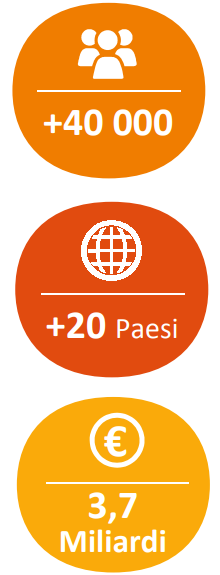
\includegraphics[width=0.6\textwidth]{immagini/dipendenti_paesi_fatturato_mondo}
\caption{Dati generali Sopra Steria nel Mondo}
\end{minipage}%
\hspace{10mm}%
\begin{minipage}[c]{.40\textwidth}
\centering\setlength{\captionmargin}{0pt}%
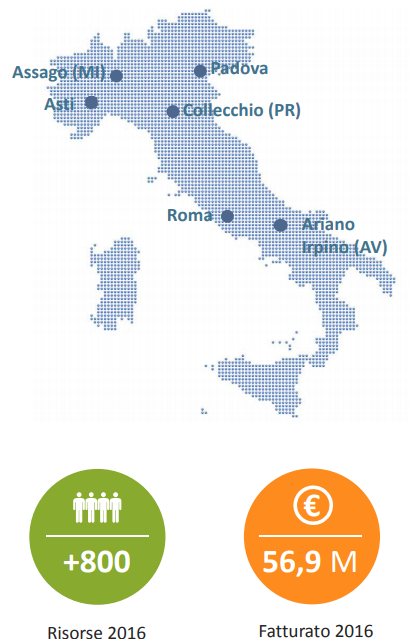
\includegraphics[width=1.2\textwidth]{immagini/mappa_italia_fatturato}
\caption{Dati generali Sopra Steria in Italia}
\end{minipage}
\caption{Informazioni generali Sopra Steria Group S.p.A. - Fonte: documento interno aziendale}
\end{figure}


Il gruppo è il risultato di una fusione avvenuta nel 2014 ad opera di due aziende, Sopra Group SA e Groupe Steria SCA, comunemente chiamate Sopra e Steria, fondate rispettivamente nel 1968 e 1969. Ad oggi l'azienda si presenta internamente ben strutturata in \textit{Business Unit}\footnote{Da questo punto per indicare il termine \textit{Business Unit} userò a volte anche il corrispettivo termine in italiano, ovvero Divisione.} relative agli ambiti di sviluppo e adotta una politica di \textit{recruiting} che mira alla competenza dei dipendenti da cui deriva la qualità dei prodotti, punto di forza dell'azienda.\\

Io sono stato inserito nella divisione "793 - Servizi Finanziari e Assicurazioni" della sede di Padova, nata negli ultimi anni a partire da pochi dipendenti e che ora conta circa 20 dipendenti solo per la sede in cui ho avuto il piacere di collaborare, senza contare i colleghi situati nelle sedi di Collecchio e Roma che cooperano anch'essi agli stessi progetti per la stessa divisione.\\
In particolare il mio ruolo è stato quello del sviluppatore \textit{host} e Analista Funzionale. \\
	Sono stato affiancato quindi da vari colleghi a seconda della tecnologia o conoscenza che dovevo apprendere. Più nello specifico sono stato affiancato dal mio collega Stefano Gori e dal mio tutor aziendale Marco Valentino, uno dei principali sviluppatori \textit{host} e manager di prossimità di questa sede, per l'apprendimento dei linguaggi COBOL\glossario\ e JCL\glossario. Sono stato invece affiancato dalle mie colleghe Chiara Maccotta e Francesca Constantini per l'apprendimento dei concetti teorici in ambito economico.\\ % essenziali per poter aver un quadro generale di quale sia lo scopo pratico del prodotto su cui si lavora e di una base teorica che permetta di raggionare sui risultati ottenuti dopo implementazioni e rispettivi risultati ottenuti.
	
	In quella che è la struttura aziendale i due ruoli per cui sono stato formato, ovvero quello di sviluppatore \textit{host} e Analista Funzionale, sono due mansioni a stretto contatto, in certi casi ricopribili ibridamente anche dallo stesso soggetto. \\ Più nel dettaglio l'incarico di Analista Funzionale consiste nel raccogliere i requisiti del cliente, tramite incontri ed interviste, ed il relazionarsi con esso al fine di capire ciò di cui ha bisogno. Con la redazione dei vari documenti di analisi questa figura deve essere in grado di portare all'interno del gruppo di sviluppo tutte le informazioni necessarie e sufficienti al successo della soluzione che verrà adottata. Nel contesto aziendale e di progetto in cui sono stato inserito io, avendo a che fare con istituti di credito, chi ricopre questo ruolo generalmente ha un \textit{background} più economico che tecnico, o in alternativa ha una pluriennale esperienza come sviluppatore tale per cui riesce comunque a tradurre le nozioni finanziarie in nozioni tecniche indirizzate agli sviluppatori. \\ Per quanto riguarda la mansione di sviluppatore \textit{host} invece consiste nel tradurre ciò che elaborano gli analisti in soluzione software mediante applicazioni in linguaggio COBOL. Generalmente chi ricopre questo ruolo ha un \textit{background} più tecnico che economico.\footnote{Da questo punto le descrizioni delle caratteristiche aziendali faranno riferimento alla \textit{Business Unit} in cui sono stato inserito, ovvero la "793 - Servizi Finanziari e Assicurazioni". Questo dato che ognuna di esse opera secondo logiche, ambiti e tecnologie differenti.}


%**************************************************************
\section{Prodotti e servizi offerti}
	
	\subsection{Prodotti}
	
	Nei mercati francesi, dove l'azienda è radicata, è attiva la vendita di prodotti bancari già pronti e configurabili in poco tempo presso i clienti. In Italia la situazione è differente e per i principali clienti, nell'ambito finanziario, raramente si vendono pacchetti di prodotti finiti ma si adotta una politica di personalizzazione secondo le esigenze del cliente. I prodotti principali offerti dalla \textit{Business Unit} in cui sono stato formato sono quindi riassumibili in:
		
	\begin{itemize}
		\item Applicazioni \textit{web} per la gestione di finanziamenti bancari, assieme alla relativa evoluzione e manutenzione;
		\item Programmi \textit{host} di gestione dati, gestione dei calcoli assieme alla consistenza e persistenza dei dati che vengono elaborati;
		\item Applicazioni \textit{web} utilizzabili dalla clientela degli istituti di credito.
	\end{itemize}
	
	\subsection{Servizi}
	
	Il sistema di gestione per la qualità dei servizi offerti ai clienti di Sopra Steria Group è certificato ISO 9001:2015 ed è annualmente sottoposto a verifiche da parte di un ente accreditato di terza parte.\\

	\begin{figure}[H]
	\centering
   	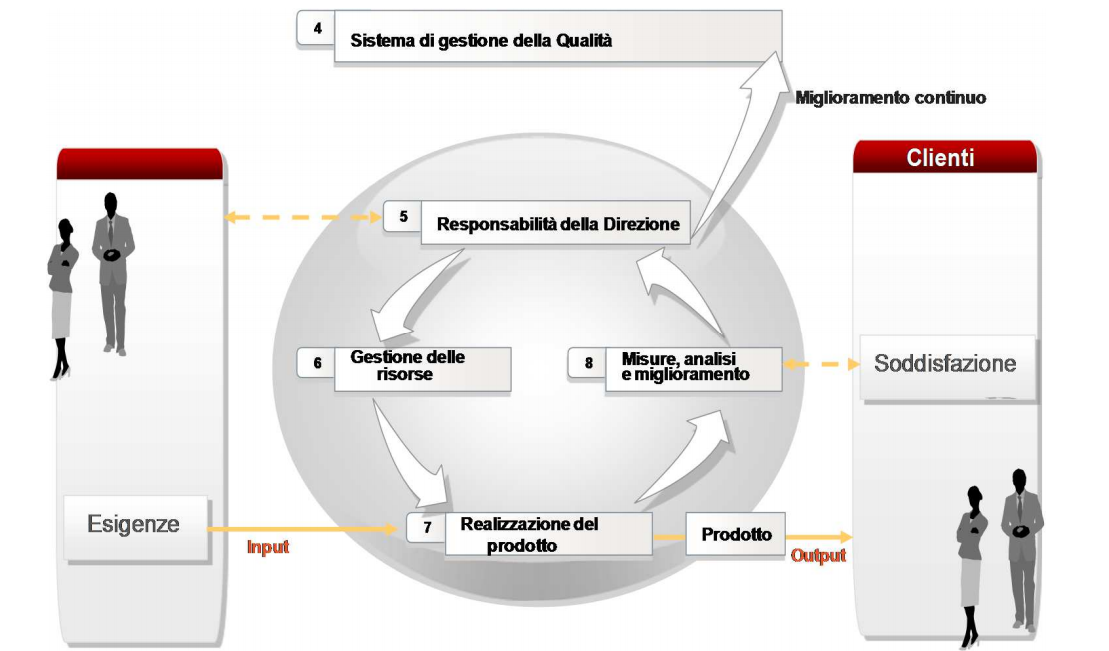
\includegraphics[width=0.85\textwidth]{immagini/ISO9001}
   	\caption{Politica della qualità di Sopra Steria Group S.p.A. - Fonte: documento interno aziendale}
	\end{figure}
	
	
	I principali servizi erogati dalla divisione per i clienti sono:
	
	\begin{itemize}
		\item Consulenza in ambito informatico per l'ampliamento ed il soddisfacimento della clientela da parte dei commerciali;
		\item Analisi delle necessità del cliente e dei conseguenti requisiti software;
		\item Progettazione e realizzazione di nuove applicazioni o nuove funzionalità di applicativi già in uso;
		\item Verifica e collaudo del software prodotto con finale rilascio nei sistemi del cliente;
		%\item Manutenzione dei contenuti proposti al cliente in un'ottica a lungo termine;
		\item Formazione del personale utilizzatore del prodotto, in particolare in seguito al rilascio di nuove funzionalità;
		\item Assistenza degli istituti bancari in caso si verifichi qualsiasi tipo di problema inerente al prodotto fornito.
	\end{itemize}	 

%**************************************************************
%\newpage
\section{Processi aziendali}

	\subsection{Organizzazione interna}
	
	L'organizzazione interna di Sopra Steria Group S.p.A. è un'organizzazione prettamente gerarchica	 che si sviluppa non solo a livello di direzione e sedi italiane ma a livello mondiale. Infatti le grandi dimensioni dell'azienda implicano questa forte strutturazione interna, assieme ad un'attenta gestione delle attività di coordinamento. Durante lo stage ho avuto modo di osservare molti degli aspetti di questo complesso sistema, anche inizialmente con la richiesta di tirocinio, che ho visto risalire lungo la gerarchia piramidale sino al consenso del direttore di \textit{Business Unit} e poi ritornare a livelli più bassi, dove una delle assistenti delle risorse umane mi ha notificato l'accettazione della richiesta.\\
	
	Una delle prime cose che si imparano di quest'azienda è la sua propensione alla cura dei rapporti con il cliente, poiché vengono offerte numerose sessioni	di consulenza. La filosofia è quella di collaborare per aiutarli a trasformare i loro sistemi informativi e, grazie all'esperienza del settore, offrire valore aggiunto mediante le soluzioni. Per raggiungere tale scopo il gruppo ha stretto delle \textit{partnership} strategiche con Microsoft, IBM, Oracle e HP. La missione principale del gruppo è di industrializzare e ottimizzare le proprie operazioni per migliorare la competitività e le  \textit{performance} in un'ottica a lungo termine.\\
	
	Un altro aspetto a cui l'azienda tiene in particolar modo è la gestione delle risorse umane. Sostenere lo sviluppo dell'evoluzione di queste ultime è considerata una priorità per il successo aziendale e per mantenere un alto livello di soddisfazione e di motivazione dei dipendenti. Per questo Sopra Steria si impegna a conoscere i profili e le competenze di ciascun collaboratore, al fine di poter offrire agli stessi prospettive di crescita e percorsi di carriera in grado di soddisfare sia le loro aspettative che il mercato. A tale scopo l'azienda organizza annualmente il cosiddetto PAP, acronimo che sta per \textit{Plan Annuel de Progression} ovvero Piano di Progressione Annuale, che serve appunto a favorire la crescita delle risorse; durante questo evento infatti i dipendenti vengono esaminati seguendo uno schema ben preciso e se le conoscenze dimostrate sono tali da potersi assumere responsabilità più grandi, questa possibilità di crescita viene valutata. Il colloquio PAP permette inoltre al collaboratore e al suo manager di prossimità di fare un bilancio del periodo appena trascorso e di fissare gli obiettivi e il piano di crescita per l'anno a venire. Durante questo evento si ha anche la possibilità di evidenziare l'esigenza di formazione e di accompagnamento per una gestione coerente della carriera. Il piano di crescita così elaborato rappresenta un impegno reciproco assunto dal collaboratore e dal suo superiore.% Fase importante della vita professionale, il colloquio PAP è un momento privilegiato di dialogo con l'azienda attraverso delle figure di riferimento, quali i Manager di Prossimità.\\
	
	%La crescente complessità dei progetti, la molteplicità degli interlocutori e le esigenze di alto livello dei clienti sono tali da comportare rischi considerevoli per l'azienda. L'intervento della direzione legale si rende pertanto necessario per difendere al meglio gli interessi del gruppo, tutelando i rapporti contrattuali con i clienti e le fasi di contenzioso, i rapporti con le software house, le parti terze, i partner e i fornitori e le acquisizioni o cessioni di attività.
	
	Per quanto riguarda il governo e la gestione del gruppo, i diversi livelli di poteri decisionali, sia a livello funzionale che produttivo, sono distribuiti nella gerarchia operativa oltre che nella direzione. Alla base di ciò, un'organizzazione complessa si ramifica nelle varie nazioni in cui l'azienda si estende, delegando l'amministrazione di questi filoni e di altri reparti di supporto a manager selezionati. A livello più basso si collocano le \textit{Business Unit}, ovvero le varie divisioni aziendali adibite all'erogazione di determinate tipologie di prodotti e servizi identificate anche in base al mercato di riferimento. Anche queste ultime risultano distribuite nel territorio, in ogni filiale infatti possono coesistere più reparti.\\
	
	\begin{figure}[H]
	\centering
	   	\includegraphics[width=0.8\textwidth]{immagini/Mercati_Principali}
	   	\caption{Suddivisione aree di mercato dell'azienda - Fonte dati: documento interno aziendale}
	\end{figure}
	
	Nella divisione in cui sono stato collocato vi sono diverse figure che si occupano dei vari processi di produzione. In ordine gerarchico è presente un direttore di \textit{Business Unit} per l'amministrazione delle risorse della divisione, i \textit{Project Manager} per la gestione dei progetti e dei loro costi, gli Analisti Commerciali che si occupano delle relazioni con i clienti, i team di Analisti e Consulenti che si occupano dei requisiti del cliente e i team di sviluppo software, suddivisi in sviluppatori \textit{web} e sviluppatori \textit{host}.\\

	%\subsection{Modello Incrementale}
	\subsection{Ciclo di sviluppo}
	
	Il ciclo di sviluppo software adottato da Sopra Steria nella divisione "793 - Servizi Finanziari e Assicurazioni" dove sono stato inserito è un'implementazione del modello incrementale, questa scelta è dovuta al fatto che l'azienda tratta per la maggior parte dei casi progetti di grandi dimensioni, il più delle volte progetti già avviati, che richiedono aggiunte sulla base delle funzionalità essenziali già sviluppate. Questo modello si caratterizza inoltre per la capacità di adattamento a molteplici tipologie di problemi.\\
	
	I punti di forza del procedimento incrementale sono i seguenti:
	\begin{itemize}
		\item L'integrazione delle parti del sistema è distribuita nel tempo e non collassata nelle fasi finali;
		\item La suddivisione in sottoinsiemi della realizzazione del problema comporta una migliore conoscenza di esso e una sua gestione più semplificata;
		\item Ogni incremento porta valore aggiunto, con lo sviluppo di nuove funzionalità e il soddisfacimento di alcuni requisiti;
		\item Ad ogni incremento si guadagnano esperienza e affidabilità, riducendo i rischi di fallimento;
		\item Le funzionalità essenziali sono sviluppate nei primi incrementi e attraversano più fasi di verifica, diventano quindi più stabili con ciascuna iterazione; questo sistema di \textit{rilasci multipli e successivi} permette anche al proponente di seguire in maniera attiva la prosecuzione del progetto avendo un'idea concreta del prodotto in corso di sviluppo.
	\end{itemize}
	
	 Questo modello si caratterizza inoltre per la capacità di adattamento a molteplici tipologie di problemi, in aggiunta si presta bene alle necessità dell'azienda perché i clienti richiedono che vengano effettuati lavori di manutenzione e amplificazione definibili in attività distinte, assimilabili facilmente tramite un ciclo di sviluppo ad incrementi. In figura vengono rappresentate le fasi del modello.\\
	
	\begin{figure}[H]
		\centering
	   	%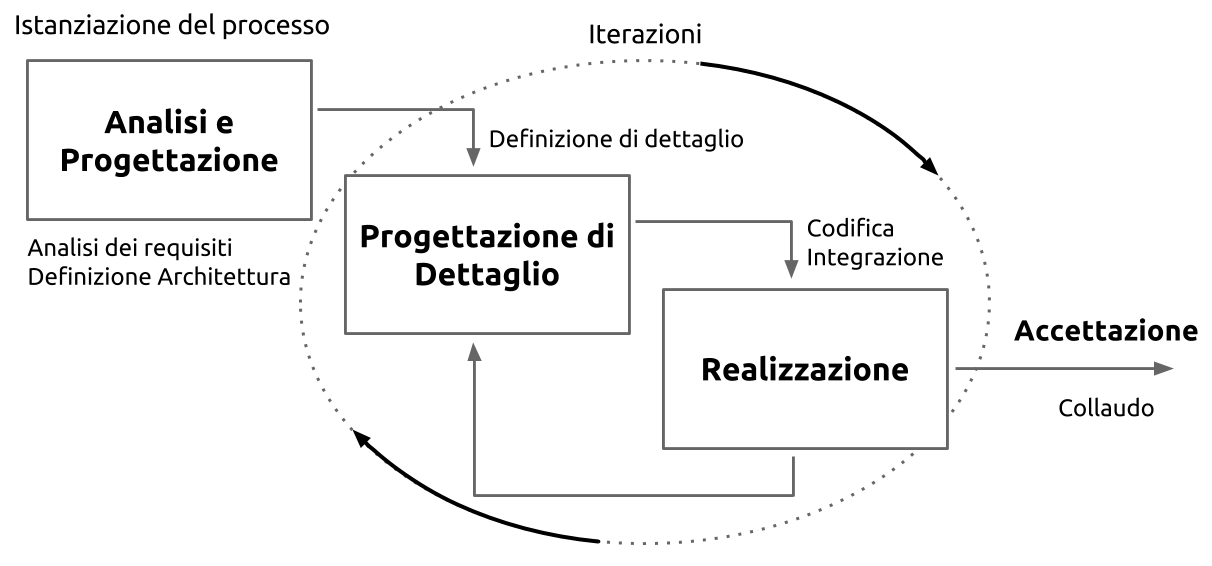
\includegraphics[width=1\textwidth]{immagini/modello_incrementale}
	   	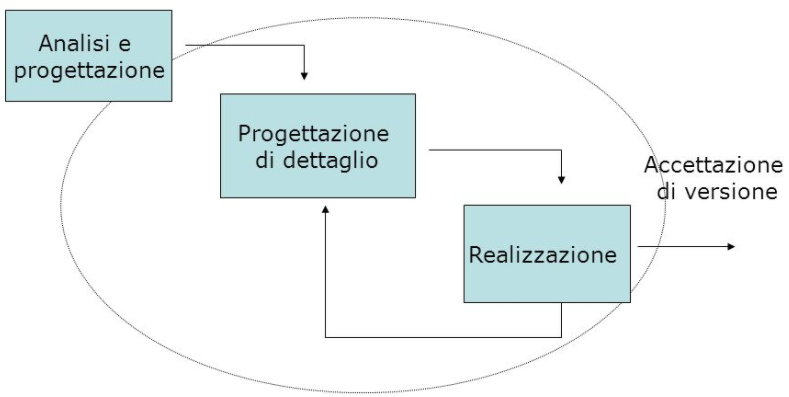
\includegraphics[width=1\textwidth]{immagini/ModelloIncrementale}
	   	%\caption{Modello di sviluppo incrementale}
	   	\caption{Modello di sviluppo incrementale - Fonte: \url{https://goo.gl/ZcNU8P}}
	\end{figure}
	%\newpage
	
	Il modello incrementale è un ciclo di sviluppo definito dallo standard ISO 12207 che combina la logica del modello a cascata, dove ogni fase è rigidamente sequenziale, e la filosofia iterativa della prototipazione.\\
	
	È prevista una prima fase di analisi dei requisiti fondamentali e di progettazione architetturale intesa a stabilire le fondamenta del software. Tale fase è essenziale per definire i successivi incrementi e non si ripete.\\
	
	Le fasi successive di realizzazione incrementale vera e propria, possono ripetersi più volte e mirano ad attività di progettazione di dettaglio, codifica e test, in cui vengono trattati prima i requisiti obbligatori, poi quelli facoltativi passando per quelli desiderabili. Le implementazioni subiscono i trattamenti di integrazione e collaudo, successivamente avviene un eventuale rilascio.\\

	È prevista la prototipazione delle nuove funzionalità che si vanno ad implementare per la validazione complessiva del sistema, reiterando 
	alle fasi di progettazione e realizzazione in caso di errori o problematiche. In questo modo è possibile di volta in volta acquisire maggiore competenza riguardo al problema, riducendo i rischi successivi e le tempistiche globali di produzione software.
	
	%\subsection{}
	\paragraph{Il modello incrementale in Sopra Steria}
\leavevmode	\newline \newline
	Ogni ciclo di incremento inizia con la raccolta e l'analisi dei requisiti presso il cliente, che espone le sue necessità tramite riunioni oppure mediante opportuna documentazione.\\
	
	Questo procedimento di raccolta dei requisiti e stesura dei documenti di analisi avviene generalmente dalle figure di Analisti Funzionali. Questi si occupano di raggruppare i requisiti in macro attività, calcolare le tempistiche necessarie per il loro completamento e stilare i documenti di \textit{Analisi Funzionale}. Dopo la stesura di tale documento, questo viene esposto al proponente al fine di approvazione. In caso il cliente ritenga che questo documento non sia adatto alle richieste o che ci siano delle mancanze viene notificato e gli analisti provvedono alle dovute correzioni. Questo procedimento di correzione della documentazione e attesa di approvazione può ripetersi sino alla giunta dell'accettazione da parte del proponente.\\
	
	Una volta approvato il documento entra in gioco la figura del \textit{Responsabile Commerciale} che presenta ai clienti un preventivo per l'implementazione delle funzionalità richieste.\\ %Pure questo preventivo passa all'approvazione del proponente e solo
	
	Una volta ottenuta l'accettazione dell'offerta commerciale si da il via alla stesura del documento di \textit{Analisi Tecnica} in cui si evince la progettazione di dettaglio. Tale documentazione risulta necessaria ai vari team di sviluppo per la comprensione e l'applicazione delle implementazioni richieste, ma non indispensabile per alcuni di essi.\\
		
	Gli analisti rimangono a disposizione degli sviluppatori anche nelle fasi successive per eventuali chiarimenti e specificazioni, in modo da non rallentare o interrompere le fasi successive. I documenti vengono inviati ai team competenti a cui sono state attribuite le macro attività e da quel momento inizia la realizzazione. Tali gruppi di lavoro possono risultare distribuiti nelle varie sedi del territorio italiano, perciò sono previste molte comunicazioni telefoniche o tramite posta elettronica e occasionali trasferte, al fine di allineare le procedure di sviluppo o rendere noto quando è possibile procedere con determinate modifiche. \\
	
	L'evoluzione degli incrementi software attraversa ambienti distinti. Esistono in particolare i seguenti ambienti:
	\begin{itemize}
		\item \textbf{Sviluppo}: ambiente di programmazione locale, qui avviene l'implementazione delle modifiche software;
		\item \textbf{Integrazione}: in questo ambiente vengono raccolte le implementazioni delle attività e si verifica che non generino conflitti, mediante test di non regressione\footnote{Con test di non regressione si intendono i test tali per cui si prova che, in eseguito alla modifica di una parte P del sistema S, la modifica di P non abbia introdotto errori né in P né alle altre parti di S che hanno relazione con P.}, garantendo la stabilità del sistema;
		\item \textbf{Collaudo}: ambiente di validazione delle funzionalità complessive del software, utilizzato anche per dimostrare al cliente la loro consistenza;
		\item \textbf{Produzione}: questo ambiente varia per ogni cliente o applicazione sviluppata e rappresenta lo stato finale del prodotto in cui viene effettivamente utilizzato dal cliente.
	\end{itemize}	
	
	È responsabilità del programmatore che prende in carico lo sviluppo delle funzionalità dichiarare il loro completamento, almeno a livello di prototipo, per rilasciarlo in integrazione. Determinati team si occupano poi di testare l'applicazione nelle sue nuove funzioni, accertando il soddisfacimento dei requisiti ed eventualmente contattando gli analisti per eventuali modifiche progettuali. In caso di problematiche le modifiche vengono respinte in ambito di sviluppo altrimenti vengono approvate per il collaudo. In collaudo è possibile utilizzare le funzioni sviluppate da altri team e validare il lavoro svolto per presentarlo poi al cliente, rilasciando in produzione la nuova versione del software.
	
	%\subsection{Strumenti a supporto di processi e servizi}
	\subsection{Tecnologie e strumenti a supporto di processi e servizi}

	Nel corso dello stage sono stati utilizzati numerosi strumenti di supporto per facilitare lo svolgimento delle diverse attività, dai tool di gestione delle basi di dati all'analisi del codice scritto passando per la gestione di progetto. Al fine di fornire ai suoi collaboratori tutti gli strumenti utili a rendere al meglio, Sopra Steria Group fornisce un portale da cui chiunque può scaricare o richiedere uno strumento, debitamente giustificato; tutto ciò affinché persista un alto livello di soddisfacimento e di motivazione dei dipendenti, che come abbiamo detto parlando di organizzazione interna è un punto sul quale l'azienda conta molto. Il portale porta il nome di \textbf{IT CORP} che abbinato al portale principale aziendale denominato Face2Face e il servizio sottostante di IT Request permettono di ottenere in qualsiasi momento applicativi o qualsivoglia strumento necessario nell'ambiente lavorativo.

	\begin{figure}[H]
		\centering
	   	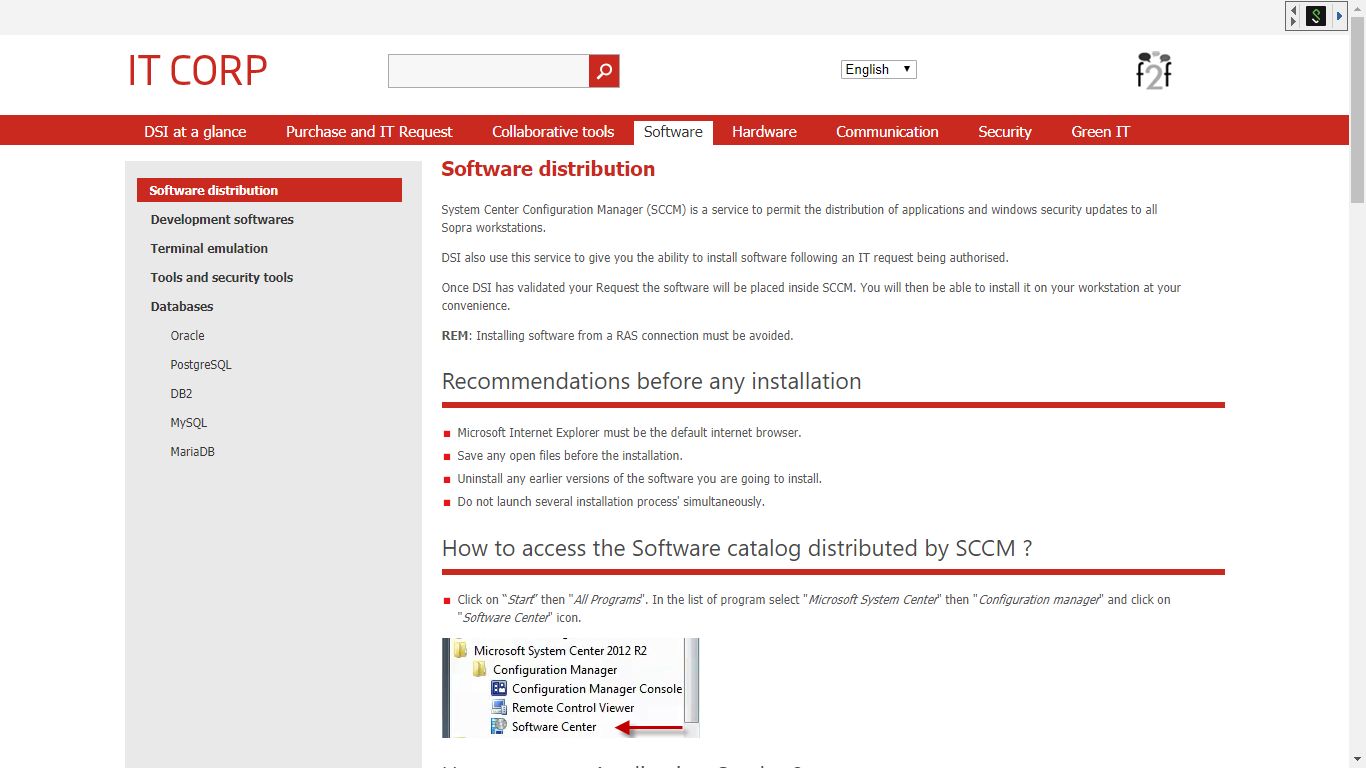
\includegraphics[width=1\textwidth]{immagini/ITCorp}
	   	\caption{La pagina iniziale di IT CORP - Fonte: Portale interno dell'azienda}
	\end{figure}
	
	La scelta degli strumenti è basata sulla pluriennale esperienza del team, che ha scelto gli strumenti con cura, dopo un attento studio delle funzionalità offerte di ognuno, attenendosi a vari fattori tra cui il supporto presente online e facilità di utilizzo, in modo da assicurare un'alta qualità dei processi. Di seguito saranno descritte le principali funzionalità e caratteristiche dei vari strumenti.\\

	Parlando di ambiente lavorativo della divisione "793 - Servizi Finanziari e Assicurazioni" e strumenti a supporto di processi e servizi all'interno di essa non si può non distinguere inizialmente e prima di tutto le due macrocategorie di ruoli che un dipendente di questa \textit{Business Unit} può assumere, ovvero la categoria degli sviluppatori \textit{Web} e quella degli sviluppatori \textit{Host}. Ognuna di queste due famiglie opera secondo politiche diverse, utilizzando processi e strumenti ben distinti. Di seguito quindi saranno descritte le principali funzionalità e caratteristiche dei vari strumenti specificando se si tratta di uno strumento a supporto della prima categoria di sviluppatori o della seconda.
	
	\subsubsection{Linguaggi}
	
	I linguaggi di programmazione utilizzati dagli sviluppatori facenti parte della divisione dove sono stato inserito sono molteplici, essendo che quest'ultima lavora su vari progetti in distinte sedi italiane. Discuterò quindi solo delle tecnologie utilizzate all'interno del progetto su cui lavora il team di cui ho fatto parte durante lo stage.
		
	\subsubsection{Linguaggi lato Host}
	\label{Linguaggi lato Host}
	Durante il periodo di stage gran parte delle attività di formazione si sono concentrate sui linguaggi da usare lato \textit{host}, ovvero i linguaggi COBOL e JCL.\\
	
	Il linguaggio \textbf{COBOL} è un linguaggio che risale agli ultimi anni '50, il suo nome è un acronimo che sta per COmmon Business-Oriented Language. Come si capisce dal nome esteso questo linguaggio è prettamente orientato al business, la traduzione del nome esteso infatti è "\textit{linguaggio comune orientato alle applicazioni commerciali}", e questo è infatti l'uso che se ne fa generalmente, ovvero programmi di gestione di sistemi bancari e assicurativi.\\

	I principali vantaggi di cui godeva il COBOL rispetto ai linguaggi che gli facevano concorrenza al tempo sono stati: 
	\begin{itemize}
		\item L'aritmetica con il punto decimale fisso, fattore molto utile nei programmi con funzioni di contabilità, che troviamo molto nel dominio bancario e in quello delle assicurazioni;
		\item Una maggiore velocità di input/output;
		\item Una sintassi con un'ottima leggibilità, conferita dal fatto che è simile a quella della lingua inglese;
		\item La capacità di gestione di enormi volumi di elaborazione con facilità.
	\end{itemize}		

	Con lo sviluppo e il perfezionarsi di questo linguaggio versione per versione, si è giunti a quella del 2002 con la quale il COBOL subiva una svolta significativa, ovvero il supporto della programmazione orientata agli oggetti.\\
	 
	Il linguaggio \textbf{JCL}, invece, è un linguaggio che anch'esso risale alla seconda metà del XX secolo ed è un acronimo che sta per Job Control Language. Il JCL è un linguaggio di \textit{scripting} generalmente utilizzato nei sistemi operativi IBM per eseguire (in gergo lanciare) una procedura batch\glossario\ su un sistema in genere mainframe. Nello specifico, lo scopo del JCL è quello di dire quali programmi eseguire, usando quali file di input e quali generare in output. L'uso che se ne fa nel contesto aziendale in cui sono stato inserito è principalmente quello di programmare e regolare l'esecuzione di programmi che generalmente vengono eseguiti periodicamente.

	\subsubsection{Linguaggi lato Web}

	Dovendo sviluppare anche l'applicativo web gli sviluppatori web su questo
fronte hanno scelto di adottare la piattaforma Java per il web (\textbf{Java EE}) e ovviamente le tecnologie standard relative alla presentazione e al comportamento delle pagine, ovvero \textbf{HTML}, \textbf{CSS} e \textbf{JavaScript}.\\

\begin{figure}[htbp]
\centering
\begin{minipage}[c]{.40\textwidth}
\centering\setlength{\captionmargin}{0pt}%
\captionsetup{width=1.2\linewidth}

\includegraphics[width=0.7\textwidth]{immagini/JavaEE}
\caption{Logo Java EE - Fonte: \url{https://goo.gl/wckR1M}}
\end{minipage}%
\hspace{15mm}%
\begin{minipage}[c]{.40\textwidth}
\centering\setlength{\captionmargin}{0pt}%
\captionsetup{width=1.25\linewidth}

\includegraphics[width=1\textwidth]{immagini/HTML5_CSS_JavaScript}
\caption{Logo HTML5, CSS3 e \\JavaScript - Fonte:\\ \url{https://goo.gl/A72tDP}}
\end{minipage}
\caption{Tecnologie utilizzate dagli sviluppatori Web}
\end{figure}
		
	L'edizione di Java che utilizzano gli sviluppatori Web è Java Platform Enterprise Edition, comunemente chiamata Java EE, che è un'estensione di Java SE (Standard Edition) e rappresenta una piattaforma di sviluppo software molto usata per applicazioni d'impresa.\\
	
	La versione di HTML utilizzata invece è la HTML5, che è l'ultima \textit{release} di HTML, risponde alle esigenze moderne ed alle aspettative dei siti web. Una delle caratteristiche principali di questa ultima edizione è il concetto di markup semantico, ovvero la capacità di fornire informazioni sul contenuto che descrive un dato tag. Oltre a questa particolarità, un'altra qualità che spicca è la capacità di adattarsi perfettamente, ovvero ad avere il medesimo comportamento sia su desktop che su mobile. \\
	
	Per tutti questi aspetti HTML5 è diventando un nuovo standard per gli sviluppatori web, tant'è che è diventato \textit{W3C Recommendation} dall'ottobre 2014.\\

	Per quanto riguarda il comportamento delle pagine web invece si è optato per l'uso della versione CSS3 per la gestione della formattazione delle pagine e di JavaScript per le validazioni e controlli \textit{client-side}.
		
	\subsubsection{Database}
	Il salvataggio dei dati per le applicazioni in ambito bancario e assicurativo avviene generalmente tramite DBMS\glossario\ relazionali come DB2 di IBM, Microsoft SQL Server e MySQL di Oracle. Il team di sviluppo in base anche ai calcolatori a disposizione della banca, anch'essi della IBM, ha scelto di utilizzare il \textbf{DB2}, che è nato nel 1983 ma tutt'oggi è uno tra gli RDBMS\glossario\ più usati, specie in questo settore. In origine era nato come DBMS per i mainframe CICS\glossario\, poi si è diffuso su diversi tipi di server. Per questo banche e assicurazioni, enti che esistono da molto prima della nascita del DB2, inizialmente hanno adottato questa tecnologia mediante sistemi EIS\glossario\ implementati in linguaggio COBOL che tutt'oggi gli forniscono le funzionalità necessarie senza il bisogno di adottare tecnologie più moderne e sviluppate secondo le esigenze dei più recenti paradigmi di programmazione.\\
	
	L'amministrazione delle basi di dati avviene tramite uno strumento denominato \textbf{DBeaver}, che è un applicazione gratuita multipiattaforma per sviluppatori, programmatori, amministratori di dabases e analisti.%Supporta più tipologie di database come MySQL, PostgreSQL, Oracle, DB2, SQL Server, MS Access e molti altri.% Teradata, SQLite, Sybase, Firebird, MariaDB, Derby 

	\begin{figure}[H]
	\centering
	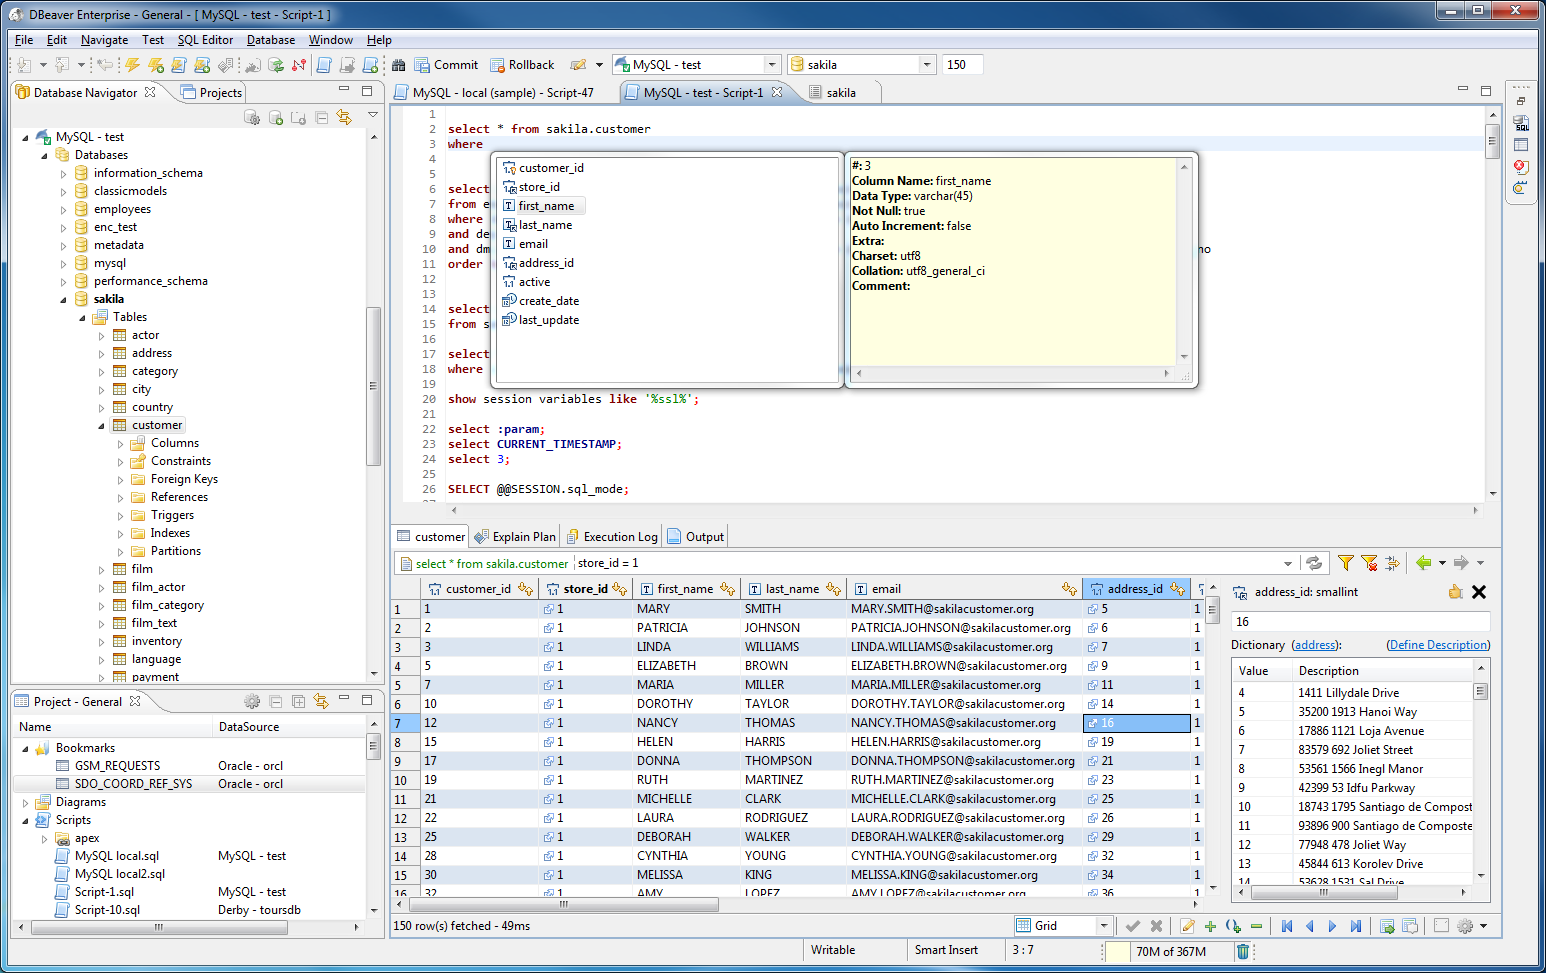
\includegraphics[width=0.85\textwidth]{immagini/DBeaver_ss}
	\caption{Schermata dello strumento di amministrazione dei databases DBeaver - Fonte: \url{https://github.com/serge-rider/dbeaver}}
	\end{figure}

	\subsubsection{Ambienti di sviluppo ed emulatori}
	\label{Ambienti di sviluppo ed emulatori}

	Anche parlando di ambienti di sviluppo è importante distinguere quelli usati lato sviluppatori \textit{web} e quelli usati lato sviluppatori \textit{host}.\\
		
	Il principale ambiente di sviluppo adottato per le applicazioni web è \textbf{Eclipse}. Esso racchiude la globalità delle caratteristiche necessarie ad uno sviluppatore in questo ambito. Rappresenta un'ottima soluzione e agevolazione per il processo di sviluppo, in quanto offre funzionalità di collegamento ai sistemi di versionamento, \textit{debugging} del codice \textit{runtime}, oltre alle molteplici caratteristiche offerte dai comuni editor di testo orientati allo sviluppo dei sorgenti software.\\
	
%	\begin{figure}[H]
%		\centering
%	   	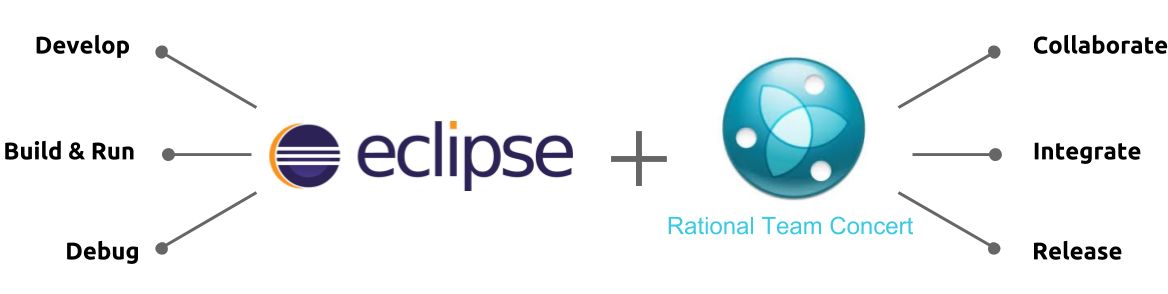
\includegraphics[width=0.7\textwidth]{immagini/ambienti_sviluppo}
%	   	\caption{I vantaggi dell'uso di Eclipse in collaborazione con RTC}
%	\end{figure}
	
	Altri programmi di supporto sono invece i diversi browser in cui bisogna testare il funzionamento delle pagine web tra cui Internet Explorer, Firefox e Chrome e gli editor di testo utili in situazioni dov'è richiesta più praticità come Notepad++.\\

	Il principale ambiente di sviluppo adottato lato \textit{host} invece è \textbf{ISPF}\glossario. Esso include vari tool e funzionalità per la gestione dell'intero processo di sviluppo dei programmi \textit{host}; dalla creazione dei programmi al versionamento degli stessi, dall'analisi statica del software in fase di compilazione alla gestione della base di dati tramite lo strumento QMF\glossario.

	\begin{figure}[H]
		\centering
	   	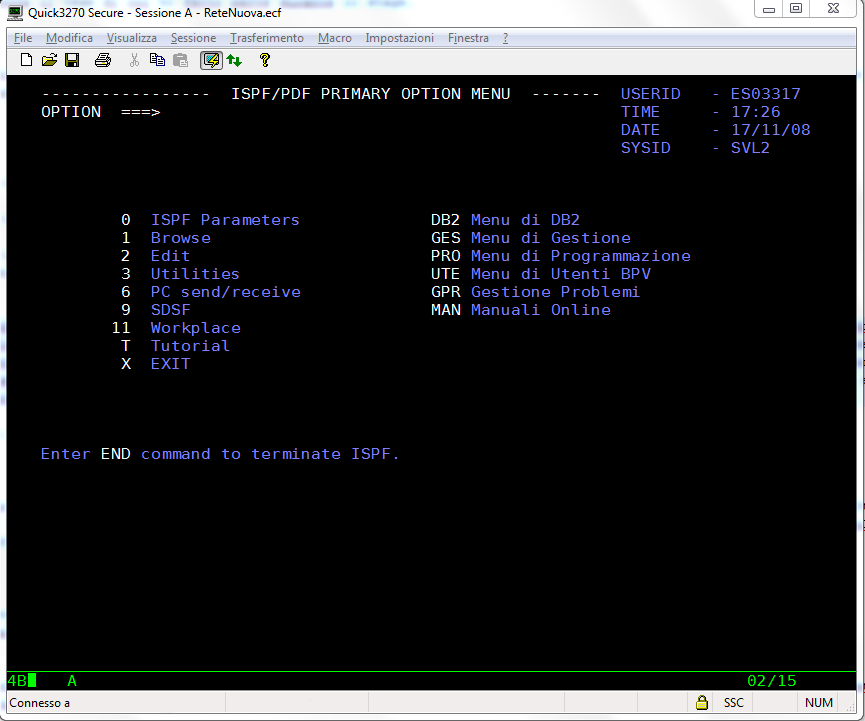
\includegraphics[width=0.80\textwidth]{immagini/ISPF}
	   	\caption{Schermata iniziale ambiente di sviluppo ISPF}
	\end{figure}

	Durante il periodo di stage ho avuto modo di imparare ad usare gran parte dei \textit{tool} che mette a disposizione ISPF, assistendo anche all'utilizzo di alcune funzionalità a cui sono abilitate solo un determinato tipo di utenze, ovvero le cosidette \textit{utenze di produzione}, che sono quelle con il totale accesso anche ai database e ai sistemi collocati dal cliente, e non solo a quelli di test su cui lavorano il resto degli sviluppatori.\\
	
	La struttura del menu di questo ambiente di sviluppo è indicativamente come illustrato nel seguente schema:
	
	\begin{figure}[H]
		\centering
		\captionsetup{width=0.70\linewidth}
	   	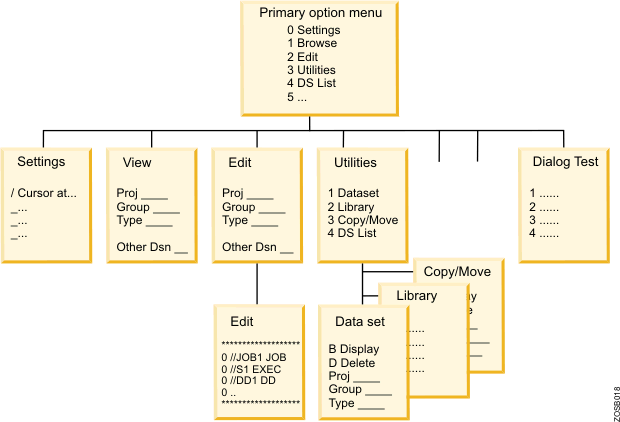
\includegraphics[width=0.80\textwidth]{immagini/ISPF_menu_structure}
	   	\caption{Struttura menu ambiente di sviluppo ISPF - Fonte: \url{https://goo.gl/GX6P9V}}
	\end{figure}

	Per utilizzare ISPF in azienda ho utilizzato l'emulatore \textbf{Quick3270 Secure} che è un potente ed affidabile emulatore di terminali IBM 3270 e IBM 5250. Utilizzabile su sistemi operativi Windows questo programma permette infatti di connettere il proprio computer ai sistemi IBM zSeries (S/390) e iSeries (AS/400).

	\subsubsection{Gestione di progetto}

	A supporto della gestione delle attività progettuali Sopra Steria mette a disposizione dei suoi dipendenti un portale comune che permette la gestione dei gruppi di lavoro. Oltre alle funzionalità di gestione di progetto questo portale permette anche l'organizzazione della comunità aziendale e favorisce il dialogo organizzato dipendente-azienda, seppur virtuale.\\
	
	Il portale aziendale, \textbf{Face2Face}, gestisce molteplici attività e problematiche. Tramite esso i dipendenti sono tenuti a riportare settimanalmente le proprie attività di lavoro e gli ambiti di progetto al fine di inviare i dati alla direzione, permettendole di coordinare le risorse a disposizione. Lo strumento consente inoltre di consultare le news aziendali e gli eventi organizzati.

	\begin{figure}[H]
		\centering
	   	\includegraphics[width=1\textwidth]{immagini/Face2Face}
	   	\caption{La Home Page di Face2Face - Fonte: portale interno dell'azienda}
	\end{figure}
		
	Face2Face è accessibile anche dall'esterno della rete aziendale tramite un portale online predisposto dall'azienda. In questo modo viene facilitato il lavoro in trasferta dei dipendenti.\\
	
	\subsubsection{Documentazione}
	\label{Documentazione}
	
	Nell'arco della mia permanenza in azienda per lo stage ho avuto modo di vedere quella che è la documentazione che la prassi aziendale vuole che venga redatta. Per ogni attività risultante dall'analisi dei requisiti, infatti, vengono stilati due documenti: l'\textit{Analisi Funzionale} e l'\textit{Analisi Tecnica}. In fase di rilascio delle funzionalità richieste durante la fase di analisi vengono redatti invece i documenti di \textit{Collaudo} e quello di \textit{Rilascio}.\\
	
	Il primo documento, ovvero quello di Analisi Funzionale, affronta i requisiti ad alto livello, enunciando le principali funzionalità ed i cambiamenti rispetto alla versione attualmente in produzione dell'applicativo.\\
	
	\leavevmode	\newline

	Le sezioni principali di questo documento sono:
\begin{itemize}
	\item Matrice dei requisiti: enunciato discorsivo per introdurre il problema proposto;
	\item Descrizione funzionale: per spiegare il comportamento dell'applicativo lato web, presentando possibilmente anche un'anteprima delle pagine che verranno aggiunte;
	\item Casi oggetto di collaudo: qui vengono indicate le componenti che saranno analizzate in fase di  \textit{testing} per verificarne il corretto comportamento;
	\item Dettaglio tecnico: qui vengono enunciate le componenti software che saranno modificate o aggiunte, senza entrare nel dettaglio di come tali modifiche andranno apportate.
\end{itemize}

	Il secondo documento invece, ovvero quello di Analisi Tecnica, affronta nel dettaglio gli aspetti tecnici che vanno modificati o aggiunti trattando principalmente i programmi COBOL lato \textit{host}, dai quali poi anche i programmatori web possono individuare i parametri da utilizzare nelle richieste via rete per recuperare i dati e quindi allinearsi.\\
	
	Il documento di Analisi Tecnica, diversamente da quello di Analisi Funzionale non sempre viene steso visto che questo non ha obbligo di approvazione da parte del cliente e quindi, in particolari casi, gli sviluppatori con più esperienza sono in grado di progettare e sviluppare la parte tecnica in autonomia senza l'aiuto di quest'ultimo.\\
	
	Al termine dello sviluppo dei requisiti, ad avvenuta validazione, vengono inoltre redatti i documenti di Collaudo e di Rilascio, da consegnare al cliente per accertare i lavori eseguiti e il rilascio delle nuove funzionalità.\\
			
	Il software utilizzato per la produzione dei documenti è \textbf{Microsoft Word}, i cui formati sono standard sia per l'azienda che per i clienti.
	
	
	\subsubsection{Sistemi di versionamento}

	Come precedentemente accennato nella sezione riguardante gli ambienti di sviluppo [\ref{Ambienti di sviluppo ed emulatori}], lo strumento \textbf{ISPF} permette, in un certo qual modo, il versionamento dei programmi sorgenti lato \textit{host}. Questo infatti tiene traccia di ogni modifica apportata ai programmi e consente quindi di ripristinare una versione di un dato modulo utilizzando un progressivo numerico, identificativo di una certa versione del software, che si incrementa ogni qualvolta questo viene modificato e compilato.\\
	
	Per quanto riguarda il lato web, invece, nel progetto su cui lavora il team in cui sono stato inserito il sistema di versionamento del software utilizzato è \textbf{RTC} (Rational Team Concert, IBM), che è costruito su IBM Jazz, una piattaforma estensibile che aiuta i team ad integrare i task attraverso il ciclo di vita del software. RTC dispone di un'architettura client-server e permette ai team di sviluppo di tenere traccia del loro lavoro in modo intuitivo.
	
	\subsubsection{Sistemi operativi}
	
	Per le postazioni di sviluppo è previsto un sistema centralizzato di utenze a cui è attribuito un proprio ambiente di lavoro ed uno spazio assegnato a cui accedere da qualsiasi computer aziendale.\\
	
	Nelle macchine aziendali è consueto l'utilizzo di Microsoft Windows 7 come sistema operativo primario per ovviare a discrepanze nelle postazioni dei diversi dipendenti e per omogenizzare ulteriormente il processo di sviluppo. Questo comporta una buona soluzione per concentrarsi unicamente sul proprio lavoro e avere al contempo una garanzia nell'utilizzo quotidiano.
	
%**************************************************************

%\section{Clientela e trasformazione digitale}
\section{Clientela ed innovazione}

	\subsection{Clientela target}
	
	La clientela target della \textit{Business Unit} "793 - Servizi Finanziari e Assicurazioni" di Sopra Steria sono principalmente gruppi bancari e assicurativi. Essi solitamente necessitano una qualche forma di innovazione o evoluzione che gli garantisca continuità di produzione ma anche i corretti adeguamenti previsti dai cambiamenti legislativi.\\
	
	 Per permettere questo, gli analisti si incaricano di entrare in contatto con i responsabili ICT\glossario\ della società cliente, dai quali poi si ricavano le diverse richieste implementative;  che possono andare dalla variazione di qualche caratteristica alla creazione di funzionalità completamente nuove.\\

	%\subsection{Principali clienti e progetti}
	
	Visto il successo conquistato con il passare degli anni Sopra Steria Group si è sempre fatta strada tra i brand più importanti in vari settori, tra i quali i seguenti, classificati per aree di mercato.
	\begin{figure}[H]
	\centering
   	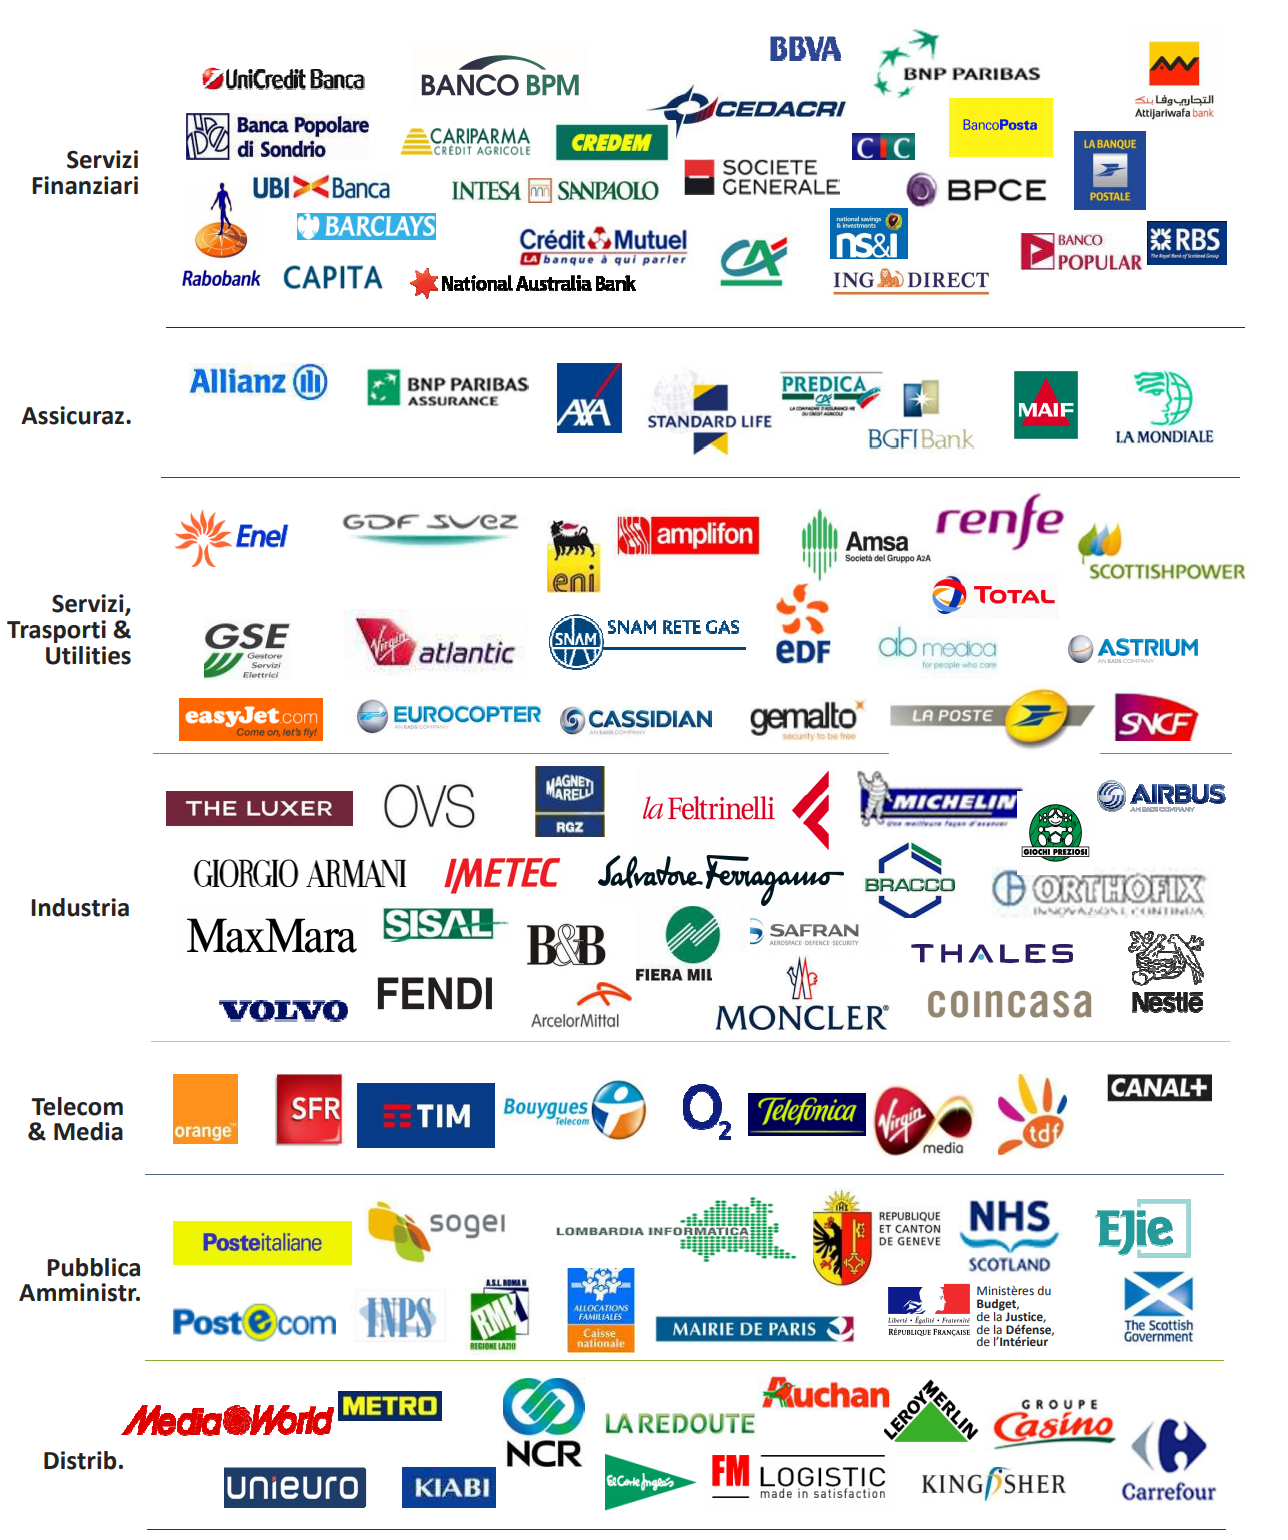
\includegraphics[width=0.7\textwidth]{immagini/principali_referenze}
   	\caption{Principali clienti di Sopra Steria Group S.p.A. - \\Fonte: documento interno aziendale}
	\end{figure}

	I progetti di maggior impatto, invece, per cui Sopra Steria è riuscita ad ottenere il privilegio di approvvigionamento e conseguente implementazione sono stati molteplici, tra questi citiamo i seguenti.
	\begin{figure}[H]
	\centering
   	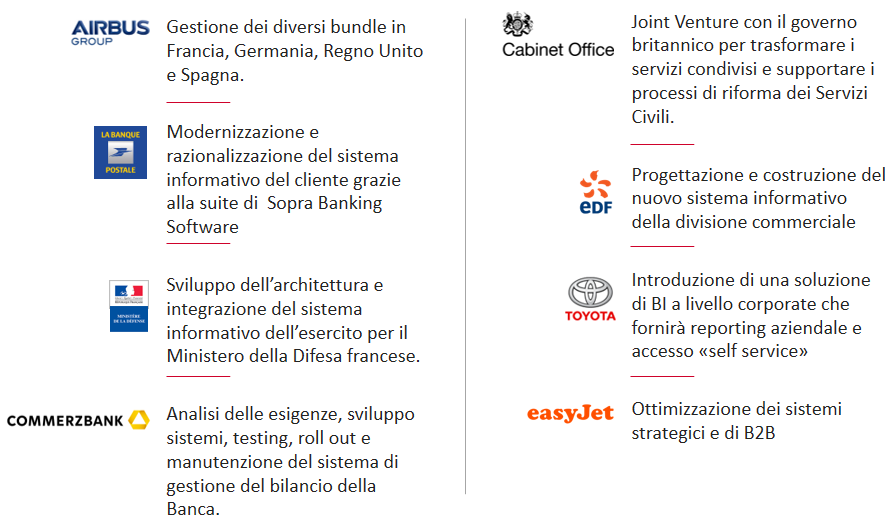
\includegraphics[width=0.76\textwidth]{immagini/Progetti_Importanti}
   	\caption{Principali progetti di Sopra Steria Group S.p.A. - \\Fonte: documento interno aziendale}
	\end{figure}

	
	\subsection{Innovazione}
	
	L'innovazione e le soluzioni software richieste dalle banche e assicurazione non sono mai stati termini accostabili. %, soprattutto negli ultimi anni.
	Se da un lato le tecnologie stanno subendo una rivoluzione importante dall'altro lato gli istituti di credito preferiscono avere sistemi funzionanti e garantiti anche se il mantenimento degli stessi richiede somme non da poco. Se da un lato si parla di migrazione sul  \textit{Cloud} dei sistemi informativi delle aziende all'avanguardia dal lato degli istituti di credito si parla al più di cambio di versione dei  \textit{Framework} utilizzati lato  \textit{front-end}\glossario.\\

	\begin{figure}[H]
	\centering
	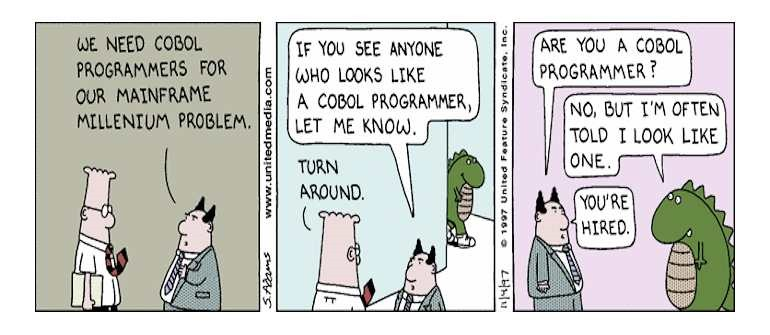
\includegraphics[width=0.85\textwidth]{immagini/VignettaCobol}
	\caption{Vignetta sull'uso del COBOL - Fonte: \url{https://goo.gl/dVnwEg}}
	\end{figure}
	
	L'innovazione in ambito bancario e assicurativo rappresenta infatti un'ostacolo non indifferente, questo tipo di enti sono da sempre legati a tecnologie primordiali come il linguaggio COBOL e la relativa implementazione in mainframe CICS.\\
	
	Per Sopra Steria, che fa della trasformazione digitale e innovazione un suo punto di forza, questo rappresenta una sfida, l'azienda infatti desidera mettersi in gioco offrendo le soluzioni adeguate, tenendo conto però delle priorità del cliente e delle sue possibilità. Queste caratteristiche sono molto ricercate dalle aziende che vogliono rinnovarsi, trasformando i loro processi e servizi nel mondo digitale, adeguandosi ai moderni canoni di utilizzo e facendosi avanti nei mercati, con la possibilità di offrire prodotti di maggiore qualità e raggiungere molti più clienti.\\
	
	Per quanto riguarda il progetto su cui lavora il team in cui sono stato inserito l'unico fattore di innovazione riguarda il lato  \textit{front-end} dell'applicazione, l'evoluzione infatti da questo lato si fa vedere mediante l'utilizzo di tecnologie moderne adatte alla presentazione dei contenuti	nel web, tecnologie che sono maggiormente soggette a spinte evolutive dovute alla modernizzazione degli standard.             % Azienda
%% !TEX encoding = UTF-8
% !TEX TS-program = pdflatex
% !TEX root = ../Lahmer_Abdelilah_tesi.tex
% !TEX spellcheck = it-IT

%**************************************************************

\chapter{La scelta del progetto}

\section{Interesse aziendale negli stage}
%In questa sezione parlerò del tipo di relazione che lega l'azienda al mondo degli stage e il loro interesse per questi. Parlerò inoltre della presenza di altri ex-stagisti che hanno fatto un mio percorso simile e sono stati assunti.

Viste le dimensioni e l'attuale espansione dell'azienda, dovuta anche al momento di buona ripresa economica che sta vivendo l'Italia, Sopra Steria Group S.p.A. è sempre più alla ricerca di nuove figure da inserire nelle proprie divisioni che operano in diversi ambiti e settori.\\

%Le modalità con cui la società attua alla ricerca di risorse sono molteplici, queste infatti possono andare dal reclutamento attraverso agenzie per il lavoro al reclutamento tramite \textit{social network} orientati al lavoro (come ad esempio LinkedIn\footnote{LinkedIn. URL: \url{https://goo.gl/nc4mVh}}), passando per il reclutamento per mezzo di eventi organizzati dalle università o dagli enti pubblici per agevolare l'incontro tra le aziende e gli studenti.\\
%
%Quest'ultimo tipo di evento rappresenta la modalità con cui sono entrato in contatto con Sopra Steria, ovvero grazie al progetto Stage-IT\footnote{Stage-IT. URL: \url{https://goo.gl/UvdwLK}}, nella sua \ang{14} edizione che si è tenuta in data 5 Aprile 2017, dove le aziende hanno avuto modo di esporre i propri progetti e gli studenti le proprie ambizioni a far parte di essi. STAGE–IT infatti è un'occasione di conoscenza reciproca per permettere agli studenti di avvicinarsi al mondo del lavoro e alle imprese di presentare la realtà in cui operano, illustrando le tematiche proposte per stage, con specifico riferimento al settore “\textit{Information and Communication Technology}" (ICT\glossario).\\
%
%	\begin{figure}[H]
%		\centering
%	   	
\includegraphics[width=0.5\textwidth]{immagini/StageIT}
%	   	\caption{StageIT 2017 - Fonte: \url{https://goo.gl/TqV3A6}}
%	\end{figure}


La politica aziendale prevede una durata di sei mesi per completare il ciclo di stage, due di questi considerati curricolari in accordo con l'Università degli Studi di Padova e quattro extracurricolari. Successivamente, nella maggior parte dei casi, vi è la propensione all'assunzione.\\%, in quanto la nuova risorsa si considera pronta per essere effettivamente inserita nei team di sviluppo o di analisi.\\

Il tirocinio è quindi visto dall'azienda come uno strumento utile a contribuire alla selezione di nuovi talenti e verificare che da entrambe le parti vi sia un interesse a proseguire il rapporto lavorativo.\\

L'interesse dell'azienda per gli stagisti e per l'incanalamento di questi nel mondo del lavoro mi è stato confermato una volta approdato nella sede per i colloqui conoscitivi, qui infatti ho avuto modo di rincontrare un collega dell'università che anch'esso aveva seguito lo stesso percorso prima di me. Questo collega infatti dopo aver concluso lo stage curricolare, conseguito la laurea ed aver concluso anche il periodo di stage extracurricolare è stato assunto a tempo indeterminato; l'unica differenza dal percorso che stavo per intraprendere io però è stata soltanto il fatto che questo collega dopo la fine dello stage bimestrale ha chiesto il cambio di \textit{Business Unit} passando alla "792 - Industria e Servizi" dove ha trovato un inquadramento come sviluppatore di applicazioni \textit{web} e \textit{mobile}. Vista questa esperienza l'impressione che l'azienda aveva trasmesso inizialmente si è sempre più confermata e personalmente guardavo con fiducia l'avvenire all'interno di Sopra Steria.

\section{Il progetto all'interno dell'azienda}
%In questa sezione parlerò del progetto che mi è stato proposto dell'azienda.

Gli stage che le aziende proponevano durante l'evento Stage-IT erano prevalentemente orientati a progetti contenuti che secondo le aziende erano fattibili nel \textit{range} di tempo che il corso di studi ci impone, ovvero un minimo di 300 ed un massimo di 320 ore.\\
	
	Dopo aver dato una buona impressione all'evento sono rimasto in contatto con l'amministrazione delle risorse umane di Sopra Steria Group S.p.A, che alla fine del mese di Aprile mi ha convocato per un colloquio collettivo assieme ad altri otto candidati. Anche in questa sede l'impressione che sono riuscito a dare e percepire da parte dell'azienda è stata più che positiva.\\
	
	% Il 17 Maggio infatti iniziavo il mio percorso presso Sopra Steria.\\ %Anche in questa sede l'impressione che sono riuscito a dare e quella che sono riuscito a percepire da parte dell'azienda è stata più che positiva. Il 17 Maggio infatti iniziavo il mio percorso presso Sopra Steria.\\

Durante il colloquio conoscitivo collettivo le domande sono state varie, in particolare una domanda ha fatto la differenza, ovvero: "Quali sono le vostre ambizioni per il futuro?". Inizialmente lo stage ideale che vedevo in azienda consisteva in un progetto nel ramo della programmazione \textit{mobile}, proiettandomi già in un ottica di stesura di una relazione di fine stage in cui sono portato a presentare un vero e proprio progetto possibilmente, che sarebbe stato sicuramente fattibile in quel ramo. La mia risposta però ha fatto sì che tutto questo venisse sconvolto. La mia replica infatti è stata grossomodo: "La mia ambizione per il futuro è quella di diventare un \textit{Project Manager} oppure un Analista Funzionale, certamente dopo aver fatto un po' di anni di gavetta per acquisire esperienza". Il colloquio collettivo infine si è concluso con la mia convocazione ad un incontro assieme al manager di prossimità della sede che mi ha illustrato in maniera generica il progetto su cui lavora il team, ovvero ELISE\glossario, e in cosa consisteva la figura di \textit{Project Manager} e Analista Funzionale in quell'ambito lavorativo. A primo impatto il ramo del \textit{banking} sembrava interessante ma rimanevo comunque aggrappato al mio stage ideale su quello del \textit{mobile}; cosa che però non ha considerato l'amministrazione delle risorse umane, che mi ha indirizzato alla \textit{Business Unit} "793 - Servizi Finanziari e Assicurazioni" con il fine di formare una figura di Analista Funzionale. Il 17 Maggio infatti iniziavo il mio percorso presso tale divisione.\\

Lo stage, quindi, così come stava per essere intrapreso, consisteva nella formazione per una mansione più che consistere in un progetto.\\

Assieme al tutor che mi era stato assegnato si sono poi decisi gli obiettivi e a grandi linee il percorso che dovevo seguire. Quest'ultimo prevedeva la mia formazione anche sulle tecnologie e modalità di sviluppo utilizzate lato \textit{back-end}\glossario\ al fine di avere un'ottica più ad ampio raggio sull'intero funzionamento del sistema, sia lato teorico che tecnico.
%Dopo una prima fase di formazione sulle tecnologie ed una di esercitazione secondo i metodi aziendali di sviluppo, quindi, il lavoro di stage si è concentrato su questo software, chiamato ELISE. Ho portato avanti il suo ampliamento aggiungendo le nuove funzionalità il cui sviluppo mi è stato assegnato.
	
%	\begin{figure}[H]
%		\centering
%	   	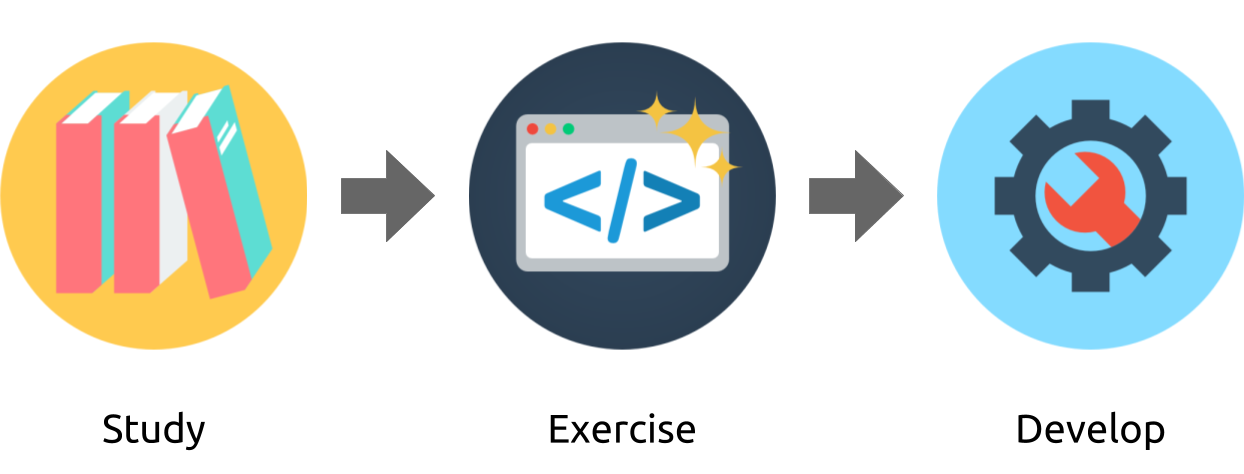
\includegraphics[width=1\textwidth]{immagini/fasi_progetto}
%	   	\caption{Le fasi principali del progetto di stage}
%	\end{figure}

\subsection{ELISE: Extended Loans Integrated System}
%In questa sezione parlerò abbastanza superficialmente del prodotto su cui la divisione in cui sono stato inserito lavora, ovvero ELISE, che è un applicazione web con scopo la gestione di finaziamenti.

	ELISE (Extended Loans Integrated System) è un software per cui la \textit{Business Unit} "793 - Servizi Finanziari e Assicurazioni" di Sopra Steria è commissionata, come molte altre aziende che forniscono consulenza nel dominio del \textit{banking}. La divisione infatti è tenuta allo sviluppo di nuove funzionalità e manutenzione su questo complesso sistema per un primario istituto di credito sul territorio nazionale, ovvero Banco BPM \footnote{Banco BPM. URL: \url{https://goo.gl/WkP9t6}}, gruppo bancario di origine cooperativa, presente in tutta Italia con l'eccezione dell'Alto Adige, operativo dal \ang{1} gennaio 2017. Questo istituto finanziario infatti è il risultato di una fusione di due grandi banche popolari, Banco Popolare di Verona e Banca Popolare di Milano, trasformatesi in S.p.A a partire dalla data di combinazione.\\

	\begin{figure}[H]
		\centering
	   	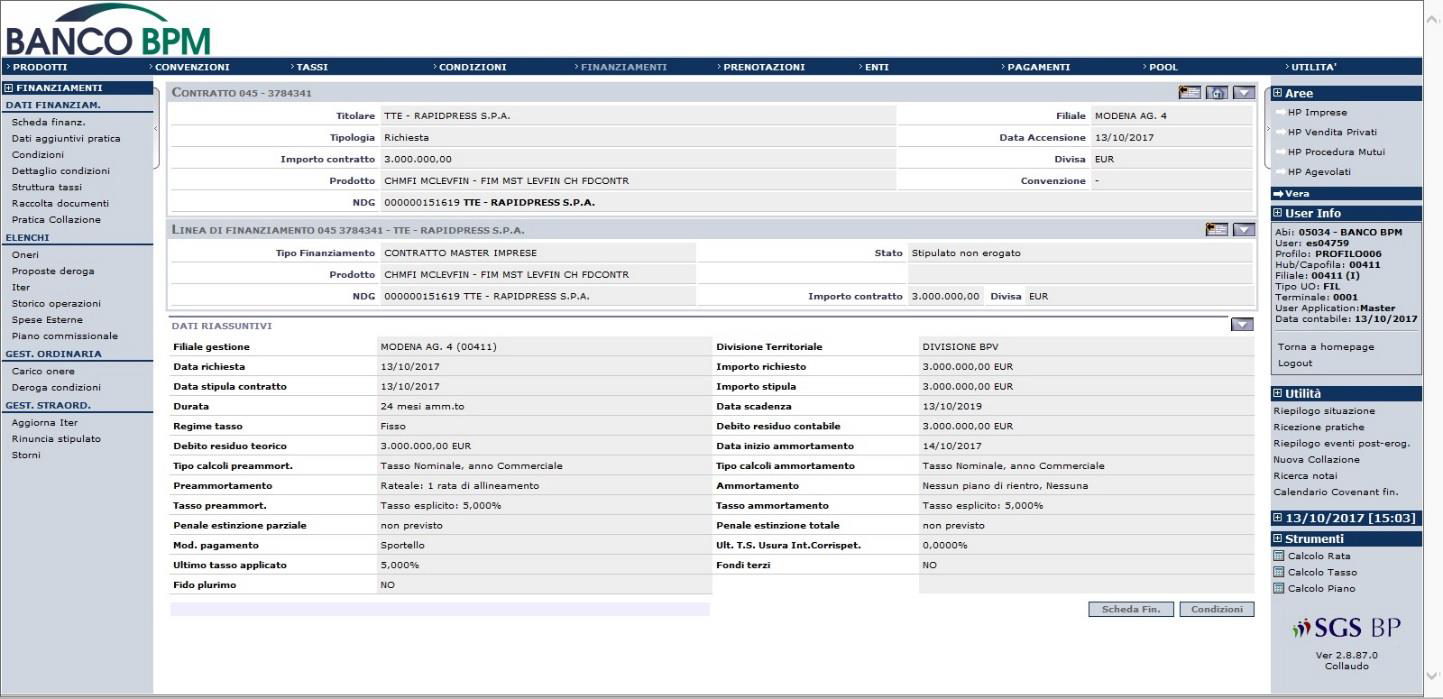
\includegraphics[width=0.85\textwidth]{immagini/Elise}
	   	\caption{Interfaccia dell'applicazione ELISE - Fonte: documento di collaudo interno aziendale}
	\end{figure}

	ELISE fornisce un ambiente completo che permette il tracciamento di un finanziamento da quando questo viene istanziato alla sua estinzione.\\
	
	ELISE si basa su un accesso ad utenza a cui sono predisposte delle abilitazioni. Ogni utente appartiene ad una filiale operativa e risulta responsabile di determinate attività da svolgere mediante l'applicazione, come ad esempio la richiesta finanziamenti, la verifica della documentazione, la gestione delle pratiche, le estinzioni, il pagamento rate, ecc. Normalmente gli utenti hanno solo determinate funzioni abilitate per sicurezza, la sede centrale invece possiede tutti i privilegi di operatività.\\
	
	I sistemi informativi di produzione in cui risiede l'applicazione web, sono in gestione presso una società ICT\glossario\ di terze parti. Tramite i loro server, il software è configurato alla comunicazione con un altro ambiente, quello di gestione dei dati, implementato su mainframe CICS\glossario\ basato appunto sulle transazioni dati.\\
		
%	\begin{figure}[H]
%		\centering
%	   	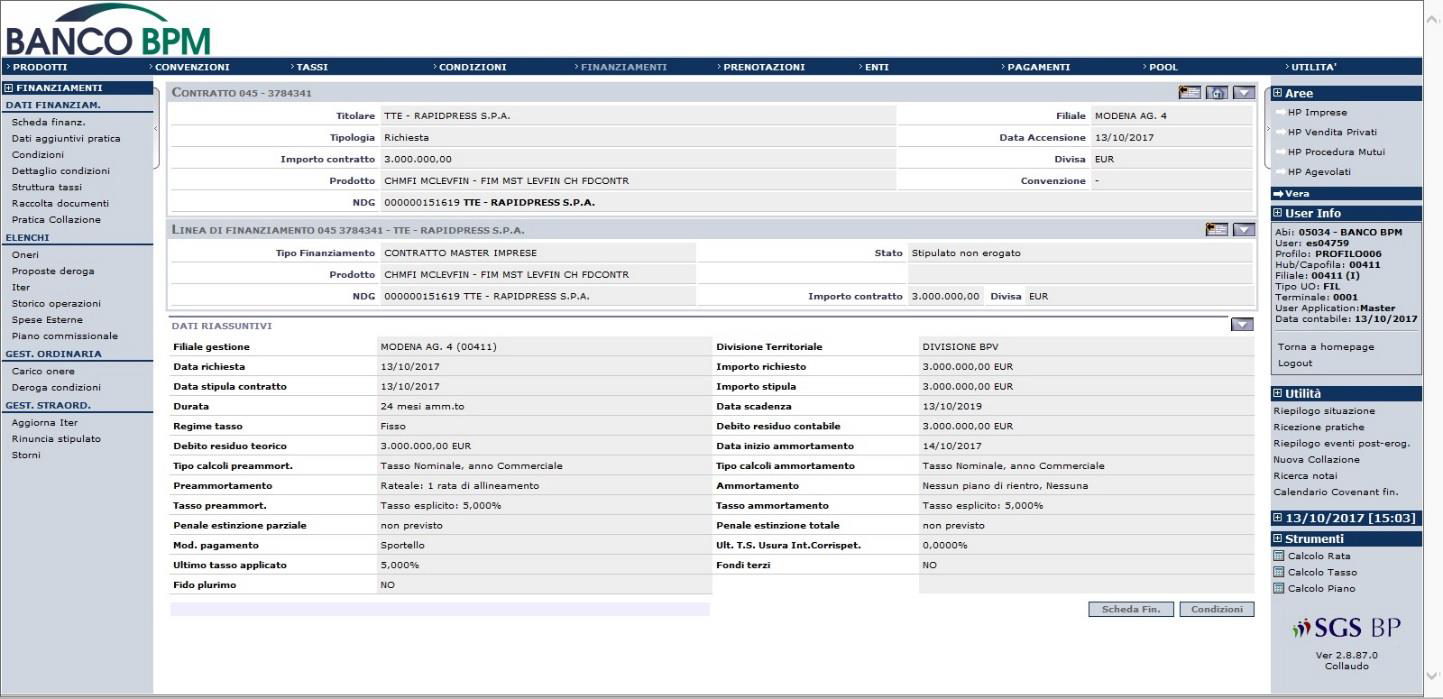
\includegraphics[width=0.85\textwidth]{immagini/Elise}
%	   	\caption{Interfaccia dell'applicazione ELISE - Fonte: documento di collaudo interno aziendale}
%	\end{figure}
	
	L'applicazione web offre, come principale strumento a supporto dei processi della banca, molteplici funzionalità, tra le più rilevanti:
	
	\begin{itemize}
		\item Prenotazione di finanziamenti sulla base dei tassi in vigore e dei dati forniti in input;
		\item Stipula dei contratti finanziari producendo in automatico come output l'accordo sottoscrivibile;
		%\item Richiesta di attivazione di un nuovo finanziamento a partire da uno prenotato; 
		\item Gestione di un finanziamento nei suoi passi, che fanno parte di quello che in ELISE viene chiamato \textit{iter pratica}, dalla prenotazione all'estinzione. Ciascuno di questi passi può essere abilitato solo per selezionate filiali della banca o tipologie di utenze;
		\item Gestione dei prodotti finanziari e dei loro parametri di periodicità, rateizzazione e spese di gestione da proporre ai clienti del gruppo bancario;
		\item Gestione dei tassi da applicare ai finanziamenti e della loro struttura fissa o variabile;
		%\item Gestione delle convenzioni stipulate per enti i cui parametri finanziari differiscono dal comune;
		\item Accesso a numerose utilità di amministrazione come il calcolo di rate, tassi o piani di ammortamento\footnote{L'ammortamento è un procedimento contabile con il quale un costo pluriennale viene ripartito tra gli esercizi di vita utile del bene, facendolo partecipare per quote alla determinazione del reddito dei singoli esercizi. Nel nostro contesto rappresenta il piano di rateizzazione per il rientro del debito residuo sommato agli interessi calcolati}.	
	\end{itemize}
		
	\begin{figure}[H]
		\centering
	   	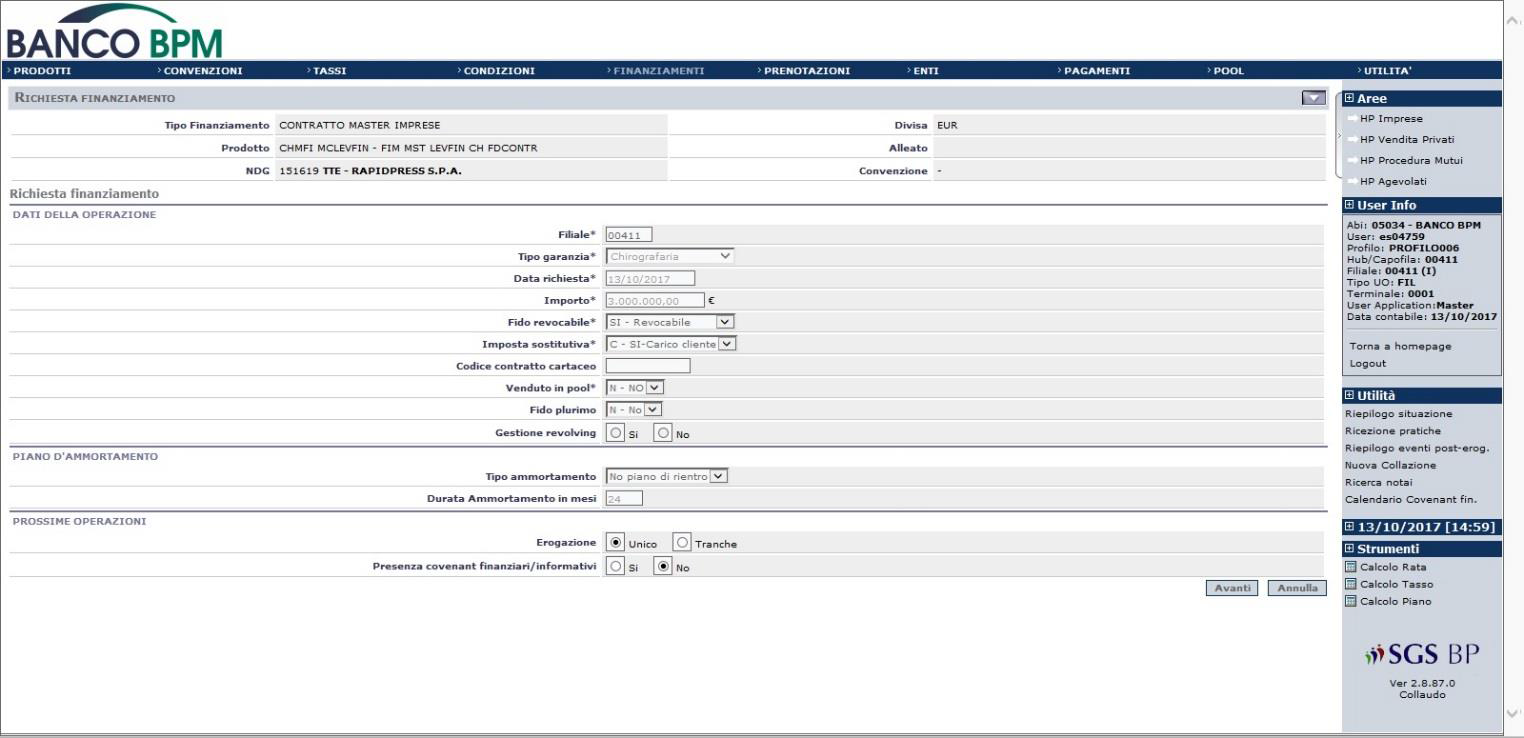
\includegraphics[width=0.85\textwidth]{immagini/RichiestaFinanziamento}
	   	\caption{Richiesta di finanziamento tramite ELISE - Fonte: documento di collaudo interno aziendale}
	\end{figure}
	
	Il portale viene utilizzato ogni giorno dai dipendenti di ogni filiale del gruppo bancario. Rappresenta quindi un mezzo di nota importanza per il cliente	e l'erogazione dei suoi servizi.

		
\section{Il mio stage}
%In questo inizio di sezione parlerò un po' di StageIT e dei progetti proposti dalle aziende in occasione di tale evento.

Le modalità con cui Sopra Steria Group S.p.A. attua alla ricerca di risorse sono molteplici, queste infatti possono andare dal reclutamento attraverso agenzie per il lavoro al reclutamento tramite \textit{social network} orientati al lavoro (come ad esempio LinkedIn\footnote{LinkedIn. URL: \url{https://goo.gl/nc4mVh}}), passando per il reclutamento per mezzo di eventi organizzati dalle università o da enti accreditati per agevolare l'incontro tra le aziende e gli studenti.\\

Quest'ultimo tipo di evento rappresenta la modalità con cui sono entrato in contatto con Sopra Steria, ovvero grazie al progetto Stage-IT\footnote{Stage-IT. URL: \url{https://goo.gl/UvdwLK}}, nella sua \ang{14} edizione che si è tenuta in data 5 Aprile 2017, dove le aziende hanno avuto modo di esporre i propri progetti e gli studenti le proprie ambizioni a far parte di essi. Stage–IT infatti è un'occasione di conoscenza reciproca per permettere agli studenti di avvicinarsi al mondo del lavoro e alle imprese di presentare la realtà in cui operano, illustrando le tematiche proposte per stage, con specifico riferimento al settore “\textit{Information and Communication Technology}" (ICT).

%	\begin{figure}[H]
%		\centering
%	   	
\includegraphics[width=0.8\textwidth]{immagini/StageIT}
%	   	\caption{Stage-IT 2017 - Fonte: \url{https://goo.gl/TqV3A6}}
%	\end{figure}

\subsection{Proposte di stage}
%In questa sottosezione parlerò delle varie proposte di stage che ho ricevuto e dei progetti che proponevano.

Nei giorni successivi all'evento Stage-IT sono stato contattato da alcune delle aziende a cui avevo fornito il mio curriculum, in particolare quelle che più hanno mostrato interesse sono state Moku SRL\footnote{Moku SRL. URL: \url{https://goo.gl/exGzcj}} e Deloitte Italy S.p.A.\footnote{Deloitte Italy S.p.A. URL: \url{https://goo.gl/cUGDsp}}, oltre a Sopra Steria Group S.p.A. naturalmente.\\

Lo stage proposto da Moku SRL consisteva in un applicazione \textit{web} nell'ambito della sanità. Questo si poneva come obiettivo, inserendo lo stagista nel team di sviluppo lato front-end\glossario, formare una figura a scopo assunzione e far sì che questa veda un progetto crescere sin dalla nascita, partendo dalla progettazione sino al rilascio, e conseguente manutenzione nel tempo. Questo progetto di stage sarebbe stato molto interessante, soprattutto per le tecnologie che avrei potuto apprendere in un ambiente giovane ed innovativo come quello delle aziende facenti parte di H-FARM\footnote{H-FARM. URL: \url{https://goo.gl/Z2RVAE}}, che è un acceleratore di \textit{startup} che negli ultimi anni si è fatto sentire molto nel campo ICT. Purtroppo non ho potuto scegliere questo progetto perché ho avuto la conferma da parte di Sopra Steria Group S.p.A. prima di quanto fatto da Moku SRL.\\
%	\begin{figure}[H]
%		\centering
%	   	
\includegraphics[width=0.3\textwidth]{immagini/moku}
%	   	\caption{Logo di Moku SRL - Fonte: \url{https://goo.gl/exGzcj}}
%	\end{figure}

Lo stage proposto da Deloitte Italy S.p.A. consisteva invece in un implementazione all'interno del prodotto Microsoft Dynamics AX\footnote{Microsoft Dynamics AX. URL: \url{https://goo.gl/1N2jsA}}, che è un ERP\glossario\ che offre tutte le funzionalità centrali per la gestione di contabilità e finanza, risorse umane e operazioni necessarie per operare e trovare clienti su scala globale. Purtroppo non ho optato per questo progetto perché la programmazione in ambito gestionali non mi ha mai appassionato, anche se l'azienda è una delle realtà più grandi su scala mondiale.\\
%	\begin{figure}[H]
%		\centering
%	   	
\includegraphics[width=0.3\textwidth]{immagini/deloitte}
%	   	\caption{Logo di Deloitte Italy S.p.A. - Fonte: \url{https://goo.gl/cUGDsp}}
%	\end{figure}

%\newpage
\subsection{Motivo della scelta}
%In questa sottosezione parlerò della scelta di stage che ho fatto e del motivo di tale scelta.

Da quando ho imboccato la strada nel dominio dell'informatica ho avuto modo di fare più di uno stage, uno dei quali con ruolo di sviluppatore. L'impressione che ho avuto dopo aver concluso queste esperienze è stata senz'altro positiva. L'esperienza che però stavo per iniziare con Sopra Steria era completamente diversa, infatti sarebbe stata la mia prima volta in un contesto di lavoro all'interno di una grande realtà del settore.\\

Per la scelta dello stage ho primariamente tenuto conto della diversa tipologia di esperienza che i progetti di stage potevano offrirmi, e Sopra Steria decisamente mi proponeva qualcosa di inusuale rispetto al comune sviluppatore che le altre aziende offrivano. Le competenze che potevo acquisire con questo progetto di stage infatti sarebbero state anche di carattere funzionale oltre a quelle di carattere tecnico.\\

Secondariamente invece ho tenuto conto delle dimensioni dell'azienda ospitante e delle possibilità all'interno di essa in un ottica a lungo termine. Sotto questo aspetto infatti Sopra Steria era stata chiara, con la grande propensione all'assunzione in seguito al semestre di stage.

\subsection{Obiettivi del progetto}
%In questa sottosezione parlerò degli obiettivi del progetto di stage che ho scelto.
All'interno del piano di lavoro relativo al periodo di stage ho stabilito degli obiettivi da raggiungere nel bimestre, obiettivi che poi sono stati riesaminati ed approvati dal tutor aziendale. La maggior parte di questi riguardano le modalità di svolgimento del lavoro in azienda, altri invece riguardano l'elaborato risultato del lavoro.\\

I requisiti sono stati suddivisi in \textbf{obbligatori}: vincolanti in quanto primari e di diretto impatto sulla valutazione dello stage; \textbf{desiderabili}: non vincolanti o strettamente necessari, ma dal riconoscibile valore aggiuntivo; \textbf{facoltativi}: rappresentanti valore aggiuntivo non strettamente necessario.

	%\subsubsection{Obbligatori}	
	\paragraph{Obbligatori}

		\begin{center}
		  \bgroup
		  \def\arraystretch{1.4}
		   \setlength\arrayrulewidth{0.6pt}
		   \begin{longtable}{ | p{11cm} |} \hline
		    \cellcolor[gray]{0.9} \textbf{Obiettivi Obbligatori} \\ \hline

			 Acquisizione di padronanza dell'ambiente di sviluppo Mainframe  \\ \hline
			 Acquisizione di padronanza delle modalità di sviluppo in ambiente Mainframe \\ \hline
			 Studio e comprensione del linguaggio COBOL\glossario \\ \hline
			 Acquisizione di padronanza di interazione con database DB2 e relativi strumenti \\ \hline
			 Implementazione di applicazioni di esempio per le funzionalità basilari \\ \hline
			 Acquisizione di padronanza d'uso di ELISE \\ \hline
			 Comprensione corretta di analisi tecniche \\ \hline
			 Integrazione nel team di sviluppo e acquisizione competenze nelle dinamiche di gruppo \\ \hline
			 Comprensione e acquisizione familiarità con la documentazione di analisi funzionale \\ \hline
			 Implementazione di modifiche basilari dell'applicazione ambito di progetto \\ \hline
			
			\caption{Tabella degli obiettivi obbligatori}
			
		    \end{longtable}
		  \egroup
		\end{center}
		
%		\begin{itemize}
%			\item Acquisizione di padronanza dell'ambiente di sviluppo Mainframe;
%			\item Acquisizione di padronanza delle modalità di sviluppo in ambiente Mainframe;
%			\item Studio e comprensione del linguaggio COBOL;
%			\item Implementazione di applicazioni di esempio per le funzionalità basilari;
%			\item Acquisizione di padronanza d'uso di ELISE;
%			\item Compresione corretta di analisi tecniche;
%			\item Integrazione nel team di sviluppo e acquisizione competenze nelle dinamiche di gruppo;
%			\item Comprensione e acquisizione familiarità con la documentazione di analisi funzionale;
%			\item Implementazione di modifiche basilari dell'applicazione ambito di progetto.
%		\end{itemize}

	\paragraph{Facoltativi}

		\begin{center}
		  \bgroup
		  \def\arraystretch{1.4}
		   \setlength\arrayrulewidth{0.6pt}
		   \begin{longtable}{ | p{11cm} |} \hline
		   
		    \cellcolor[gray]{0.9} \textbf{Obiettivi Facoltativi} \\ \hline

			Studio delle meccaniche di comunicazione con la parte \textit{web} (\textit{front-end}) dell'applicazione ELISE \\ \hline
			Rilascio di nuova funzionalità analizzata e sviluppata \\ \hline

			
			\caption{Tabella degli obiettivi facoltativi}
			
		    \end{longtable}
		  \egroup
		\end{center}	

	%\subsubsection{Desiderabili}		
	\paragraph{Desiderabili}		

		\begin{center}
		  \bgroup
		  \def\arraystretch{1.4}
		   \setlength\arrayrulewidth{0.6pt}
		   \begin{longtable}{ | p{11cm} |} \hline
		   
		    \cellcolor[gray]{0.9} \textbf{Obiettivi Desiderabili} \\ \hline

			Raggiungimento di un buon livello di autonomia nell'analisi di funzionalità \\ \hline
			Raggiungimento di un buon livello di concepimento, anche se parziale, delle modalità di traduzione delle analisi di funzionalità in analisi tecnica \\ \hline
			Capacità di portare a termine le attività lavorative secondo le tempistiche stabilite \\ \hline
			Capacità di portare a termine le attività lavorative anche in situazioni critiche \\ \hline
			Conoscenza delle norme di sicurezza relative all'ambiente di lavoro \\ \hline
			Comprensione e acquisizione familiarità con concetti teorici in ambito economico \\ \hline
			Acquisizione di padronanza delle attrezzature presenti in azienda in funzione del proprio lavoro \\ \hline
			\caption{Tabella degli obiettivi desiderabili}
		    \end{longtable}
		  \egroup
		\end{center}

	Di seguito in figura si mostra graficamente la suddivisione degli obiettivi nelle varie tipologie. Come si può notare gli obiettivi obbligatori compongono più del 50\% dei totali concordati e il restante si suddivide in desiderabili e facoltativi.\\
	
	\begin{figure}[H]
		\centering
	   	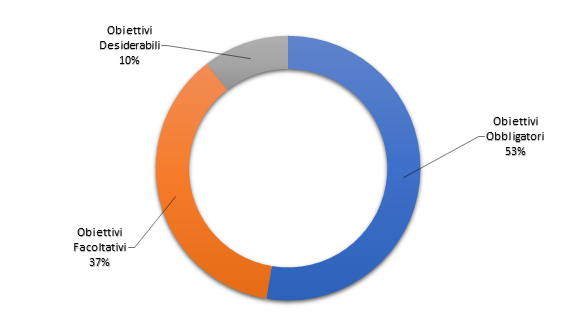
\includegraphics[width=0.5\textwidth]{immagini/Percentuale_Obiettivi}
	   	\caption{Suddivisione degli obiettivi dello stage}
	   	%\vspace{2mm}
	\end{figure}

\subsection{Vincoli del progetto}
\label{Vincoli del progetto}
%In questa sottosezione parlerò dei vincoli imposti sia dall'azienda che dal cliente per il progetto di stage che ho scelto.
	
	%\subsubsection{Imposti dal cliente}	
	\paragraph{Imposti dal cliente}
	\leavevmode	\newline
	\leavevmode	\newline
	Per quanto riguarda gli sviluppi sull'applicativo ELISE il cliente ha imposto diversi vincoli, questi però riguardano più la programmazione \textit{web} che quella \textit{host}.\\
	
	Il cliente infatti richiede che l'applicazione sia compatibile ed utilizzabile sugli elaboratori a disposizione dei suoi dipendenti nelle varie filiali; gli sviluppatori sono quindi tenuti allo sviluppo delle nuove funzionalità e alla manutenzione di quelle già in produzione tenendo conto della compatibilità di quel che producono con i browser in uso dalla banca, ovvero \textit{Internet Explorer}.\\
	
	Il cliente richiede inoltre prestazioni di utilizzo dell'applicativo, questo vincolo quindi riguarda sia gli sviluppatori \textit{host} che quelli \textit{web}, i quali devono evitare una complessità ciclomatica\footnote{Con complessità ciclomatica si intende quella del flusso di controllo, il suo valore è funzione dei possibili differenti cammini sul grafo di flusso.} troppo alta, che potrebbe portare ad un rallentamento dell'applicativo a discapito delle performance richieste.\\

	Altri vincoli sono invece più specifici e riguardano le versioni delle tecnologie da utilizzare lato \textit{front-end}, solitamente vengono applicate sempre le ultime versioni delle tecnologie possibili, cercando di contrastare, almeno da questo lato, l'arretratezza dei meccanismi di programmazione in ambito bancario.

	%\subsubsection{Imposti dall'azienda}	
	\paragraph{Imposti dall'azienda}
	\leavevmode	\newline
	\leavevmode	\newline
	Dal punto di vista dell'azienda, l'obiettivo è sempre quello di garantire al cliente il costante funzionamento del prodotto e il rispetto del contratto delle funzionalità, assieme alla consistenza e persistenza dei dati che vengono elaborati.\\
	
	Tra i vincoli imposti dall'azienda, troviamo la strutturazione del codice secondo il paradigma aziendale, in particolare per quanto riguardo il codice COBOL ogni sviluppatore è tenuto ad associare ad ogni riga di codice che produce un cosiddetto "\textit{segnalino}" per far sì che si tenga traccia dell'autore e causa di ogni modifica.\\
	
	Anche per quanto riguarda i documenti che vengono stilati dagli analisti l'azienda impone un vincolo, ovvero il rispetto della struttura e \textit{template} aziendale, per quest'ultimo Sopra Steria fornisce un estensione di Microsoft Word che favorisce il rispetto di questa condizione.

\subsection{Obiettivi personali}
\label{Obiettivi personali}
%In questa sottosezione parlerò degli obiettivi che mi sono imposto iniziando il progetto di stage.
	Con l'inizio di questa esperienza di stage le mie aspettative erano di trovare un clima lavorativo che mi insegnasse le metodologie di lavoro utilizzate in progetti di grandi dimensioni come mi era parso conoscendo l'azienda.\\

	In particolare mi aspettavo di poter contribuire senza particolari ostacoli sotto l'aspetto tecnico, avendo già basi sulle metodologie di programmazione grazie al percorso di studi offerto dall'Università, anche se applicati ad altri linguaggi di programmazione differenti dal COBOL.\\
	
	Sotto l'aspetto funzionale, invece, speravo di potermi integrare in quello che sarebbe stato un ruolo di maggiore importanza in azienda, speravo di poter iniziare a dar il mio contributo autonomamente pur non avendo basi di natura economica; per raggiungere ciò però sapevo di necessitare di formazione da parte dell'azienda.\\
	
	Desideravo formarmi professionalmente, accrescere il mio potenziale in ambito lavorativo e allo stesso tempo diventare autonomo nelle mie attività; potendo così dar manforte al team favorendo la concretizzazione di quella che era una mia ambizione.             % Progetto
%% !TEX encoding = UTF-8
% !TEX TS-program = pdflatex
% !TEX root = ../Lahmer_Abdelilah_tesi.tex
% !TEX spellcheck = it-IT

%**************************************************************
\chapter{Il progetto di Stage}

\section{Pianificazione del lavoro}
%In questo inizio di sezione parlerò della pianificazione del lavoro per il progetto di stage in fatto di tempistiche.
Per raggiungere gli obiettivi pianificati nel piano di stage e rispettare i requisiti minimi imposti dall'Università, io e il tutor aziendale abbiamo previsto 304 ore di lavoro, distribuite in circa 8 settimane da 40 ore ciascuna. Ho iniziato lo stage il 17 Maggio 2017 e terminato il 10 Luglio 2017, rimanendo in linea con quanto pianificato inizialmente, senza incorrere in particolari differimenti da quanto programmato.

\subsection{Definizione del piano di lavoro}
%In questa sottosezione parlerò della pianificazione del lavoro per il progetto di stage riportando i dati dal piano di lavoro con la programmazione delle ore da dedicare a ciascuna attività.
	Nei giorni immediatamente precedenti l'inizio dello stage mi sono recato in sede Sopra Steria e ho redatto il Piano di Lavoro, con conseguente revisione del tutor aziendale. In questo documento ho definito gli obiettivi e la pianificazione delle attività, assegnando ad ognuna una tempistica in ore e suddividendo l'intero percorso di stage in tre fasi. Ho specificato inoltre le modalità di interazione col tutor e una previsione delle competenze che sarei andato ad acquisire.\\

Tramite il Piano di Lavoro e la pianificazione dettagliata in esso avrei potuto infatti verificare l'effettivo allineamento tra il lavoro svolto e il lavoro pianificato man mano che il percorso di stage volgeva al termine.\\
	
Settimanalmente inoltre aggiornavo il mio tutor interno sulla mia situazione in relazione alla pianificazione, riportando eventuali scostamenti dal Piano di Lavoro. \\

\newpage

	Le fasi individuate in tale documento sono state:
	
	\begin{itemize}
		\item \textbf{FASE 1 - Formazione tecnica}: durante questa prima fase del percorso formativo era prevista l'introduzione alle modalità di approccio alla programmazione tramite dei corsi a seconda dell'ambiente di sviluppo, tecnologie e linguaggi di programmazione da utilizzare; in particolare era previsto: 
			\begin{itemize}
				\item lo studio e utilizzo dell'ambiente di sviluppo mainframe;
				\item lo studio dei concetti fondamentali del linguaggio di programmazione COBOL\glossario;
				\item lo studio delle modalità di interazione con database DB2;
				\item lo sviluppo di semplici programmi nell'ambito dell'applicazione realizzata da Sopra Steria.
			\end{itemize}
		\item \textbf{FASE 2 - Formazione funzionale}: durante questa seconda fase del percorso formativo era prevista l'introduzione alla metodologia di operatività in ambito funzionale, iniziando a lavorare a stretto contatto con il resto del team della \textit{Business Unit} addetta ai Servizi Finanziari. Erano previste infatti attività di formazione di carattere funzionale in ambito bancario, apprendendo la modalità di collegamento tra quella che è la parte funzionale del sistema con la parte tecnica, introdotta nella FASE 1; in particolare era previsto: 
			\begin{itemize}
				\item lo studio e utilizzo del sistema sviluppato dall'azienda, ovvero ELISE\glossario;
				\item lo studio e utilizzo della parte relativa alla funzionalità di “finanziamenti in Pool\footnote{I finanziamenti in Pool in ambito bancario rappresentano quelli che vengono denominati anche \textit{prestiti sindacati}, sono erogati da un insieme di banche a favore di un'impresa. Scopo di tale raggruppamento è la ripartizione del rischio e dello sforzo di finanziamento.}” all'interno di ELISE;
				\item lo studio delle modalità di trasformazione dei concetti funzionali in tecnici.
			\end{itemize}
		
		\item \textbf{FASE 3 - Analisi tecnica e funzionale modulo “Pool”}: In questa ultima e terza fase del percorso formativo era previsto lo studio della parte tecnica e funzionale di uno dei moduli dell'applicazione orientata ai finanziamenti realizzata da Sopra Steria, ovvero il modulo “Pool”. Era previsto inoltre lo sviluppo in linguaggio COBOL di quelle che sarebbero state le funzionalità studiate ed analizzate nel documento funzionale e tecnico.% In particolare in questa fase del percorso di stage erano previsti:
%			\begin{itemize}
%				\item lo studio e l'analisi del modulo;
%				\item la progettazione dell'analisi funzionale;
%				\item la redazione dell'analisi Funzionale e Tecnica del modulo.
%			\end{itemize}

	\end{itemize}
\leavevmode	\newline

%\newpage
		\begin{center}
		  \bgroup
		  \def\arraystretch{1.4}
		   \setlength\arrayrulewidth{0.6pt}
		   \begin{longtable}{ | p{2.61cm} | p{9cm} |} \hline
		   %\begin{longtable}{ | p{2.5cm} | p{0.5cm} | p{9cm} |} \hline
		   
		    %\cellcolor[gray]{0.9} \textbf{Durata in ore} & \cellcolor[gray]{0.9} & \cellcolor[gray]{0.9} \textbf{Descrizione dell'attività} \\ \hline
		    
		    \cellcolor[gray]{0.9} \textbf{Durata in ore} &  \cellcolor[gray]{0.9} \textbf{Descrizione dell'attività} \\ \hline


			76 	& FASE 1: FORMAZIONE TECNICA \\ \hline

			\tab \tab 24 & Formazione ambiente di sviluppo Mainframe\\
			\cline{2-2}		%\cline{2-2}
			\tab \tab 52 & Formazione linguaggio di programmazione COBOL \\	\hline
			
			76 	& FASE 2: FORMAZIONE FUNZIONALE \\ \hline

			\tab \tab 12 &  Formazione sul sistema sviluppato dall'azienda\\
			\cline{2-2}		%\cline{2-2}
			\tab \tab 12 &   Formazione sulla parte relativa al concetto di “Pool”\\
			\cline{2-2}		%\cline{2-2}
			\tab \tab 52 &  Formazione sulla modalità di trasformazione dei concetti funzionali in tecnici\\	\hline			
			
			152 & FASE 3: ANALISI TECNICA E FUNZIONALE MODULO “POOL” \\ \hline

			\tab \tab 40 &  Analisi modulo \\
			\cline{2-2}		%\cline{2-2}
			\tab \tab 40 &  Progettazione dell'analisi funzionale \\
			\cline{2-2}		%\cline{2-2}
			\tab \tab 72 &   Redazione analisi Funzionale e Tecnica modulo \\	\hline
			
			\caption{Pianificazione delle attività di stage}
			
		    \end{longtable}
		  \egroup
		\end{center}
	
\subsection{Livello di autonomia}
%In questa sottosezione parlerò del livello di autonomia con cui ho svolto lo stage.

	Inizialmente con l'inizio dello stage l'idea era quella di lavorare in un ambiente che mi teneva a stretto contatto con il tutor aziendale, in modo tale da favorire l'interazione e garantire il raggiungimento degli obiettivi prefissati, come da Piano di Lavoro; successivamente però ho scoperto che non sarebbe stato così. Il tutor aziendale infatti, essendo manager di prossimità della sede e facente parte del team degli Analisti Funzionali, era generalmente in trasferte lavorative in sedi distaccate di Sopra Steria oppure dal cliente.\\
	
	Sono stato quindi affiancato da più colleghi della sede per le diverse competenze che dovevo apprendere.\\
	
	Questo tipo di approccio però non è stato positivo; i colleghi a cui sono stato affiancato infatti, soprattutto lato tecnico non sono stati in grado di farmi seguire un percorso di apprendimento proficuo, non avendo particolari metodi di insegnamento oltre ad una visione incompleta dell'architettura dell'applicazione.\\
	
	Questo fattore è stato un deficit rilevante al fine del raggiungimento degli obiettivi prefissati.\\

	Il livello di autonomia che ho raggiunto alla fine del percorso infatti non era sufficiente da poter portare a termine un'attività di sviluppo o analisi in completa indipendenza, necessitavo infatti di saltuarie delucidazioni.\\
	
	La difficoltà di lavoro in modalità autonoma è secondariamente dovuta al fatto che l'ambiente di sviluppo mainframe era a me sconosciuto prima di iniziare l'esperienza di stage, durante il percorso di studi infatti non è mai stato possibile trattare praticamente questo tipo di contesto. La mancanza di basi di natura economica inoltre hanno sfavorito parzialmente l'autonomia sotto l'aspetto funzionale.

\section{Formazione}
%In questo inizio di sezione farò una panoramica sulla formazione che ho ricevuto, sia quella in ambito teorico-economico sia quella in ambito tecnico.

Le prime due fasi del percorso di stage le ho dedicate alla formazione in due ambiti, quello tecnico e quello funzionale. La formazione tecnica si poneva come obiettivo fornire una sufficiente base sul linguaggio di programmazione COBOL e le modalità di sviluppo, utilizzando quest'ultimo, in ambiente mainframe. La formazione funzionale, invece, si poneva come obiettivo quello di apprendimento d'uso di ELISE e dei concetti economici fondamentali utilizzati in esso.

\subsection{Conoscenze economiche acquisite}
%In questa sottosezione parlerò più approfonditamente della formazione in ambito teorico-economico che ho ricevuto e riporterò i macro argomenti trattati, magari con qualche accenno a qualche concetto fondamentale.

Come ho indicato nella sezione dedicata [\ref{ELISE: Extended Loans Integrated System}], ELISE è un complesso sistema di gestione di finanziamenti, esso infatti fornisce un ambiente completo che permette il tracciamento di un prestito da quando questo viene istanziato alla sua estinzione. I concetti di natura teorica indispensabili al concepimento degli stati in cui questo può trovarsi e delle funzionalità predisposte dall'applicazione su di esso sono stati oggetto della formazione teorica ricevuta.\\

Di seguito riporterò le più rilevanti nozioni acquisite.

\paragraph{Finanziamento}
Un finanziamento è un rapporto che intercorre tra almeno due soggetti e consiste nella cessione di una somma di denaro con il vincolo della restituzione di capitali di pari valore o maggiori.\\
Gli elementi costitutivi di un finanziamento sono:
	\begin{itemize}
		\item capitale finanziato;
		\item tasso annuo nominale d'interesse (TAN);
		\item tasso annuo effettivo globale (TAEG);
		\item durata del finanziamento;
		\item l'importo, ed eventuali rate e condizioni.	
	\end{itemize}

L'assegnazione di un prestito avviene dopo una serie di controlli preliminari che il mediatore esegue in base alla situazione economica e professionale del soggetto richiedente, esami che gli permettono di valutare la sicurezza evitando sconvenienti situazioni di insolvenza.\footnote{Wikipedia - Prestito (finanza). URL: \url{https://goo.gl/mwp69N}}

\paragraph{Fido}
Un fido bancario, o affidamento, è definito come l'impegno assunto da una banca a mettere una somma a disposizione del cliente, o di assumere per suo conto un'obbligazione nei confronti di un terzo. Un fido bancario può essere concesso sia ad un privato sia ad un'azienda, tuttavia è quest'ultima la categoria che ricorre maggiormente al credito bancario. Gli affidamenti bancari vengono concessi dagli istituti di credito a seguito di una complessa istruttoria che di norma ha ad oggetto sia i profili reddituali che quelli patrimoniali del soggetto richiedente al fine di stabilire la capacità di restituzione del credito concesso (profilo reddituale) e la solidità finanziaria (profilo patrimoniale).\footnote{Wikipedia - Fido bancario. URL: \url{https://goo.gl/49Wwbs}}

\paragraph{Tasso}
In economia, il tasso di interesse effettivo rappresenta la percentuale dell'interesse su un prestito e l'importo della remunerazione spettante al prestatore. Viene espresso come una percentuale per un dato periodo di tempo e indica quanta parte della somma prestata debba essere corrisposta come interesse al termine del tempo considerato o, da un altro punto di vista, indica il costo del denaro. Il debitore, infatti, ricevendo una somma di denaro, si impegna a pagare una somma superiore a quella ricevuta. La differenza costituisce l'interesse, che viene solitamente calcolato in percentuale sulla somma prestata. Tale percentuale costituisce il tasso di interesse. Il tasso d'interesse è variabile anche in funzione della moneta di riferimento, del rischio connesso alla solvibilità del debitore e della lunghezza del periodo di riferimento.\footnote{Wikipedia - Tasso d'interesse. URL: \url{https://goo.gl/AHpfia}}

\paragraph{Piano di ammortamento}
Il piano di ammortamento è un programma di estinzione di debito o di abbassamento o estinzione del capitale di credito. Esistono diversi tipi di piano di ammortamento:
	\begin{itemize}
		\item Ammortamento a rate costanti (francese);
		\item Ammortamento con quote capitali costanti (italiano).	
	\end{itemize}
Il piano utilizzato nel sistema bancario italiano è quello alla francese, cioè a rate costanti. Visualizzando il piano di ammortamento ci si accorge che:
	\begin{itemize}
		\item la rata è sempre la stessa (sempre che il tasso non cambi);
		\item la quota interessi è pari al tasso di interesse del periodo per il debito residuo alla fine del periodo precedente;
		\item la quota capitale è la differenza tra rata e quota interessi.\footnote{Wikipedia - Piano di ammortamento. URL: \url{https://goo.gl/vtBdix}}
	\end{itemize}

\paragraph{Finanziamento in Pool}
I prestiti sindacati, conosciuti anche come "finanziamenti in pool", sono erogati da un consorzio di banche (il pool) a favore di un'impresa. Scopo di tale raggruppamento è la ripartizione del rischio e dello sforzo di finanziamento; il pool si scioglie una volta ultimata l'operazione. I prestiti in pool fanno parte di quella categoria di finanziamenti a medio-lungo termine che concedono le banche. I prestiti in pool fanno parte di quella categoria di finanziamenti a medio-lungo termine che concedono le banche. All'interno di un pool si distingue solitamente:
	\begin{itemize}
		\item la banca \textit{arranger} che si assume l'onere dell'organizzazione (in ELISE questa si chiama banca "\textit{rappresentante}");
		\item la banca capofila, (spesso coincide con la banca \textit{arranger}) che coordina la sindacazione;
		\item la banca agente che cura tutti gli aspetti amministrativi dopo l'operatività del prestito;
		\item la banca partecipante che eroga una quota parte del prestito.\footnote{Wikipedia - Prestiti sindacati. URL: \url{https://goo.gl/nQyvFh}}
	\end{itemize}

\subsubsection{ELISE}
\label{ELISE}
%In questa sotto sottosezione descriverò ELISE e spiegherò i suoi scopi e funzionalità principali, collegando infine il tutto con le attività formazione teorico-economiche che ho applicato in essa dopo averle acquisite.

Nella formazione sotto l'aspetto funzionale uno dei principali obiettivi era anche quello di apprendere la modalità d'uso di ELISE, ovvero l'applicazione ambito di progetto aziendale. Durante questa fase di formazione ho cercato di acquisire capacità di navigazione all'interno di essa. Quest'attività di apprendimento è strettamente legata alla formazione sui concetti teorico-economici discussi nella sezione precedente.\\

Nel formarmi su questo complesso sistema ho afferrato un concetto molto importante: ELISE è un applicazione orientata ai "\textit{Prodotti di Finanziamento}", ogni prestito istanziabile infatti fa parte di un prodotto, che è visto come una tipologia di finanziamento offerto dall'istituto di credito. Ogni prodotto ha le proprie condizioni, che possono essere derogabili o meno. Tali condizioni possono variare nel tempo, per questo nel processo di richiesta di un finanziamento il prodotto viene clonato, assieme alle rispettive condizioni, al fine di salvare la versione utilizzata.\\

Le funzionalità principali di ELISE oggetto di formazione sono state:
	\begin{itemize}
	\item creazione dei vari tipi di finanziamento;
	\item pagamento rate di un dato finanziamento;
	\item estinzione di un dato finanziamento;
	\item modifica delle condizioni dei vari "Prodotti di Finanziamento";
	\item creazione di pool;
	\item creazione di finanziamenti in pool;
	\item stipula di contratti di finanziamento.
	\end{itemize}

\subsection{Tecnologie utilizzate}
%In questa sottosezione parlerò più dettagliatamente delle tecnologie che ho utilizzato.

\subsubsection{Piattaforma host}
%In questa sotto sottosezione introdurrò la piattaforma host su cui ho lavorato, spiegando nel dettaglio la struttura della rete e i vari elaboratori su cui il codice viene immagazzinato ed eseguito.

Nel formarmi sotto l'aspetto tecnico, ovvero sulle metodologie di programmazione \textit{back-end}\glossario, ho avuto modo di comprendere e avere un'idea di quella che è l'architettura della piattaforma \textit{host}.\\

Tale architettura si sviluppa su più sedi, che comprendono le diverse filiali dell'istituto di credito, assieme a quelle delle aziende di ICT\glossario\ addette alla manutenzione dei sistemi informativi della banca e dell'implementazione all'interno di essi di nuove funzionalità, com'è il caso di Sopra Steria.\\

Gli elaboratori principali, ovvero i mainframe, sono localizzati all'interno delle unità CED\glossario\ degli istituti finanziari, il colloquio con questi avviene tramite transazioni CICS\glossario\footnote{Transazioni CICS. URL: \url{https://goo.gl/QKRXTe}}, anche dagli uffici centrali delle banche che generalmente coincidono con la sede in cui questi sono installati.\\

Per lo sviluppo su questo tipo di piattaforma è necessario l'uso degli strumenti, quali emulatori e ambienti di sviluppo, illustrati nella sezione relativa alle tecnologie e strumenti a supporto di processi e servizi [\ref{Ambienti di sviluppo ed emulatori}].\\

Nel processo di rilascio di nuove funzionalità il team di sviluppatori segue un procedimento di \textit{packaging} dei sorgenti a cui sono state apportate modifiche, al fine di "\textit{portare in produzione}", in gergo, le nuove implementazioni.\\

Questo procedimento installa sull'elaboratore centrale il nuovo applicativo, effettuando un trasferimento fisico sulla macchina.\\

Di seguito riporto una raffigurazione indicativa dell'architettura su cui si basa il progetto ELISE:

	\begin{figure}[H]
		\centering
	   	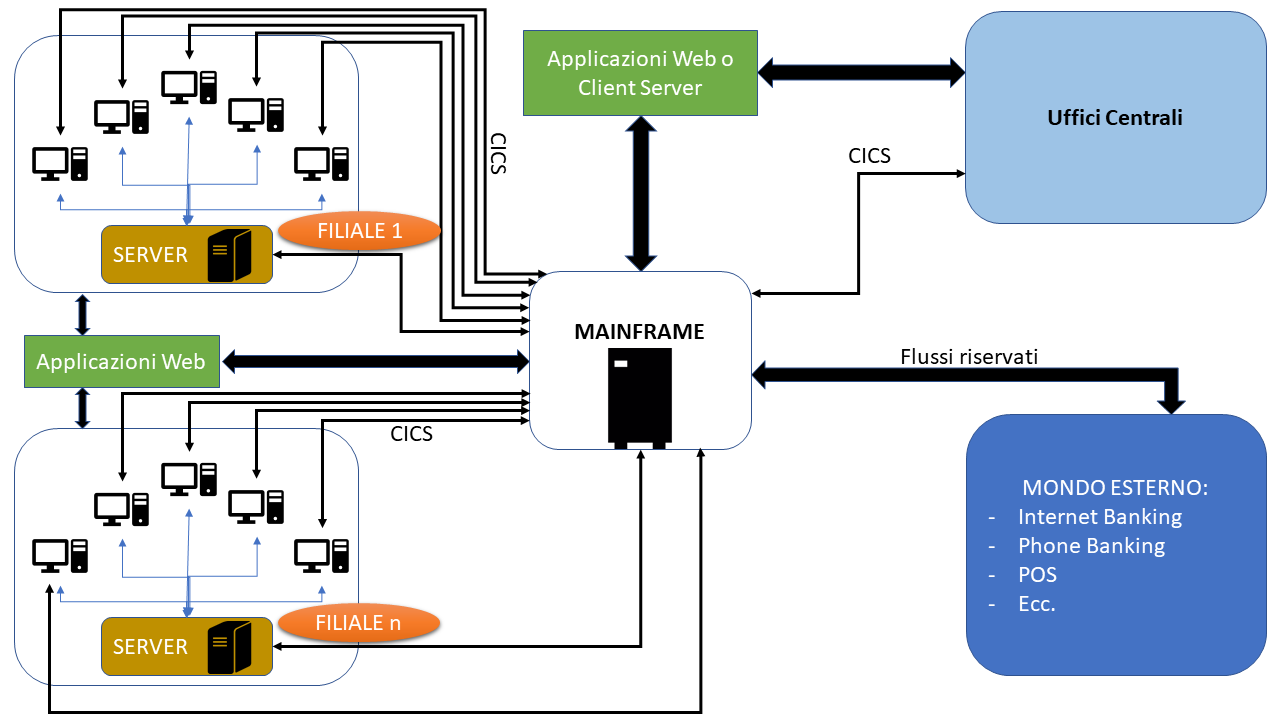
\includegraphics[width=1\textwidth]{immagini/Architettura}
	   	\caption{Architettura piattaforma Host - Fonte schema:\\ \tab \url{https://goo.gl/gZFJRF} }
	\end{figure}

	
\subsubsection{COBOL}
%In questa sotto sottosezione riporterò i concetti fondamentali di quello che è il linguaggio di programmazione COBOL e l'uso che se ne fa, riportando poi alcuni esempio dei formalismi principali tramite i quali i moduli delle applicazioni host elaborano i dati.

Durante la formazione sulla parte tecnica gran parte del tempo lo ho dedicato al linguaggio COBOL.\\

In un programma scritto in linguaggio COBOL è indispensabile, secondo la prassi aziendale, la presenza delle seguenti divisioni:
\begin{itemize}

\item \textbf{IDENTIFICATION DIVISION}: in questa divisione vengono incluse informazioni generiche come il nome del programma, la data di creazione e la funzione del programma;

\item \textbf{ENVIRONMENT DIVISION}: in questa divisione viene indicato l'ambiente in cui viene utilizzato il programma (il tipo di macchina), l'eventuale presenza di file di input-output e la modalità di controllo di questi ultimi;

\item \textbf{DATA DIVISION}: in questa divisione vengono definite le aree di variabili e costanti utilizzate all'interno del programma;

\item \textbf{LINKAGE SECTION}: in questa sezione, facente parte della DATA DIVISION, vengono definite le aree di comunicazione comuni ai moduli di ELISE, assieme alle interfacce utilizzate all'interno del programma;

\item \textbf{PROCEDURE DIVISION}: in questa divisione è definito il corpo elaborativo del programma, all'interno di questo \textit{scope} infatti viene specificato il flusso del modulo.
\end{itemize}

Di seguito riporto un frammento di codice con la struttura ideale di un programma scritto in linguaggio COBOL:

\begin{lstlisting}[language=cobol, caption={Struttura ideale di un programma COBOL}]
ABDELI IDENTIFICATION DIVISION.
ABDELI PROGRAM-ID.   ESCOBOL.
ABDELI AUTHOR.       ABDELILAH LAHMER.
ABDELI DATE-WRITTEN. 2017-12-01.
ABDELI*
ABDELI ENVIRONMENT DIVISION.
ABDELI*
ABDELI DATA DIVISION.
ABDELI*
ABDELI WORKING-STORAGE SECTION.                         
ABDELI*
ABDELI PROCEDURE DIVISION.
ABDELI*-------COMMENTO: INIZIO PROCEDURE DIVISION-------
ABDELI INIZIO-PGM.
ABDELI     DISPLAY 'INIZIO PROGRAMMA ESCOBOL'
ABDELI 	   PERFORM CORPO-PGM
ABDELI     PERFORM STAMPA-FINE
ABDELI .
ABDELI*
ABDELI CORPO-PGM.
ABDELI     DISPLAY 'ESECUZIONE CORPO PROGRAMMA ESCOBOL'.
ABDELI*
ABDELI STAMPA-FINE.
ABDELI     DISPLAY 'FINE PROGRAMMA ESCOBOL'.
ABDELI*--------COMMENTO: FINE PROCEDURE DIVISION--------
\end{lstlisting}

Come si nota dal frammento di codice precedente l'area che verrà interpretata dal compilatore va dalla ottava colonna in poi, le prime sei colonne infatti sono adibite al cosiddetto "\textit{segnalino}" (accennato nella sezione [\ref{Vincoli del progetto}]) e la settima all'eventuale commento della riga.\\

%\leavevmode	\newline

L'uso che se ne fa del COBOL nei sorgenti prodotti è principalmente quello di interfacciamento con il database, interrogandolo in lettura, modifica dei dati a seconda delle funzioni richiamate dall'utente che interagisce con l'interfaccia \textit{web} e scrittura dei dati, in caso la funzione richiamata lo richieda.\\

%\newpage
I principali costrutti indispensabili per l'elaborazione dei dati sono:

\begin{itemize}
	\item \textbf{IF}: permette di condizionare l'esecuzione di un gruppo di istruzioni;
	\begin{lstlisting}[language=cobol, caption={Esempio d'uso costrutto IF in COBOL}]
ABDELI*--------ESEMPIO USO  COSTRUTTO IF--------
ABDELI 	IF DATO-INPUT IS NUMERIC
ABDELI 	  PERFORM ELABORA-NUMERICO
ABDELI	ELSE
ABDELI	  PERFORM ELABORA-ALFANUMERICO
ABDELI	END-IF.
	\end{lstlisting}
	
	\item \textbf{PERFORM}: permette il richiamo di una funzione presente nel programma; consente infatti di eseguire un gruppo di istruzioni contenute all’interno di sezioni o di paragrafi della divisione PROCEDURE DIVISION, riprendendo poi il flusso dall'istruzione successiva;
	\begin{lstlisting}[language=cobol, caption={Esempio d'uso costrutto PERFORM in COBOL}]
ABDELI*------ESEMPIO USO COSTRUTTO PERFORM------
ABDELI FUNZIONE-CHIAMANTE.
ABDELI     DISPLAY 'FUNZIONE-CHIAMANTE'
ABDELI 	   PERFORM CHIAMA-FUN2.
ABDELI     DISPLAY 'FINE FUNZIONE-CHIAMANTE'
ABDELI*
ABDELI CHIAMA-FUN2.
ABDELI     DISPLAY 'ESECUZIONE CORPO CHIAMA-FUN2'.
	\end{lstlisting}

	\item \textbf{EVALUATE}: permette la gestione di più condizioni, specificando il modo di elaborazione di ognuno in caso si verifichi, evitando di utilizzare molteplici costrutti IF innestati;
	\begin{lstlisting}[language=cobol, caption={Esempio d'uso costrutto EVALUATE in COBOL}]
ABDELI*-----ESEMPIO USO  COSTRUTTO EVALUATE-----
ABDELI 	EVALUATE DATO-INPUT
ABDELI	  WHEN 'NUMERICO'
ABDELI 	    PERFORM ELABORA-NUMERICO
ABDELI	  WHEN 'ALFANUMERICO'
ABDELI	    PERFORM ELABORA-ALFANUMERICO
ABDELI	END-EVALUATE.
	\end{lstlisting}

\newpage

	\item \textbf{MOVE}: permette la copia o assegnazione di un valore ad una o più variabili di destinazione;
	\begin{lstlisting}[language=cobol, caption={Esempio d'uso costrutto MOVE in COBOL}]
ABDELI*-------ESEMPIO USO  COSTRUTTO MOVE-------
ABDELI MOVE ZERO		TO VAR-INDICE.
	\end{lstlisting}

%\newpage


	\item \textbf{SET}: in quel che è la prassi aziendale questo costrutto viene utilizzato per settare una variabile booleana;
	\begin{lstlisting}[language=cobol, caption={Esempio d'uso costrutto SET in COBOL}]
ABDELI*--------ESEMPIO USO COSTRUTTO SET--------
ABDELI SET FLAG		TO TRUE.
	\end{lstlisting}

	\item \textbf{VARYING}: permette la gestione di un contatore numerico specificando il valore di inizializzazione dopo il FROM, l'incremento ad ogni ciclo dopo il BY e la condizione di uscita dopo l'UNTIL, in questo modo è possibile utilizzare dei cicli di elaborazione dati in modo semplice.
	\begin{lstlisting}[language=cobol, caption={Esempio d'uso costrutto VARYING in COBOL}]	
ABDELI*------ESEMPIO USO COSTRUTTO VARYING------
ABDELI PERFORM VARYING VAR-INDICE FROM 1 BY 1
ABDELI  UNTIL VAR-INDICE > LUNGHEZZA
ABDELI   DISPLAY 'INDICE: ' VAR-INDICE
ABDELI END-PERFORM
	\end{lstlisting}
		
\end{itemize}
	
\subsubsection{JCL}
%In questa sotto sottosezione riporterò i concetti fondamentali di quello che è il linguaggio di scripting JCL e riportando qualche esempio dell'uso che se ne fa, ovvero il controllo dell'esecuzione di moduli COBOL.
Durante la formazione sulla parte tecnica ho avuto modo di operare superficialmente con il linguaggio JCL\glossario. Come accennato nella sezione relativa ai linguaggi utilizzati [\ref{Linguaggi lato Host}] il JCL è un linguaggio usato con lo scopo di dire all'elaboratore quali programmi eseguire, usando quali file di input e quali generare in output. L'uso che se ne fa in azienda consiste nel programmare e regolare l’esecuzione di programmi in modalità batch\glossario. \\

Per il JCL non è stata prevista formazione, come da Piano di Lavoro; una volta apprese le modalità di sviluppo però ne ho scoperto l'indispensabilità.\\

\newpage

Di seguito riporto un frammento di codice\footnote{JCL - Eseguire programmi COBOL. URL: \url{https://goo.gl/bpaFUC}} in linguaggio JCL che esegue il programma MYCOBB a titolo di esempio:

%\begin{lstlisting}[language=C++]
\begin{lstlisting}[language=Cobol, caption={Struttura ideale di un programma JCL}]
//STEP001  EXEC PGM=IKJEFT01
//*
//STEPLIB  DD DSN=MYDATA.URMI.DBRMLIB,DISP=SHR
//*
//input files
//output files
//SYSPRINT DD SYSOUT=*
//SYSABOUT DD SYSOUT=*
//SYSDBOUT DD SYSOUT=*
//SYSUDUMP DD SYSOUT=*
//DISPLAY  DD SYSOUT=*
//SYSOUT   DD SYSOUT=*
//SYSTSPRT DD SYSOUT=*
//SYSTSIN  DD *
    DSN SYSTEM(SSID)
    RUN PROGRAM(MYCOBB) PLAN(PLANNAME) PARM(param)
    LIB('MYDATA.URMI.LOADLIB')
    END
/*
\end{lstlisting}

\section{Processo di sviluppo}
%In questo inizio di sezione introdurrò la fase di stage relativa al processo di sviluppo del progetto di stage.
%Al termine delle prime fasi di formazione ero portato alla realizzazione di un progetto di stage che consisteva nella redazione di un'Analisi Funzionale e Tecnica del modulo "Pool", assieme all'implementazione di quanto studiato nell'Analisi Funzionale. Una volta entrato nell'ambiente lavorativo ed avuto un'idea di quella che era l'architettura di ELISE sono riuscito a concepire la difficoltà di questi compiti, sopratutto in relazione al tempo di formazione che avevo avuto. Il modulo "Pool" di cui si richiedeva l'analisi, infatti, era pressoché la metà dell'intera architettura del sistema, oltre al fatto di essere già implementato.\\
%
%Visto ciò ho scelto di analizzare un'altra funzionalità, in parte collegata al concetto di Pool, ovvero quella di "calcolo delle Commissioni di Mancato Utilizzo (CMU)"\footnote{La commissione di mancato utilizzo viene calcolata sull'importo non impiegato di un finanziamento, che però è stato predisposto dall'istituto di credito a favore del cliente; generalmente questa commissione ammonta allo 0,50\% su base annua.}, anch'essa già implementata ma solo a scopo di esercitazione mi preparavo ad esaminarla.

\subsection{Analisi dei requisiti}
%In questa sottosezione descriverò l'attività di analisi dei requisiti e riporterò il modo in cui è stata svolta.

Al termine delle prime fasi di formazione ero portato alla realizzazione di un progetto di stage che consisteva nella redazione di un'Analisi Funzionale e Tecnica del modulo "Pool", assieme all'implementazione di quanto studiato nell'Analisi Funzionale. Una volta entrato nell'ambiente lavorativo ed avuto un'idea di quella che era l'architettura di ELISE sono riuscito a concepire la difficoltà di questi compiti, sopratutto in relazione al tempo di formazione che avevo avuto. Il modulo "Pool" di cui si richiedeva l'analisi, infatti, era pressoché la metà dell'intera architettura del sistema, oltre al fatto di essere già implementato.\\

Visto ciò ho scelto di analizzare un'altra funzionalità, in parte collegata al concetto di Pool, ovvero quella di "calcolo delle Commissioni di Mancato Utilizzo (CMU)"\footnote{La commissione di mancato utilizzo viene calcolata sull'importo non impiegato di un finanziamento, che però è stato predisposto dall'istituto di credito a favore del cliente; generalmente questa commissione ammonta allo 0,50\% su base annua.}, anch'essa già implementata ma solo a scopo di esercitazione mi preparavo ad esaminarla.\\

	Come prima attività nel processo di sviluppo di nuove funzionalità l'azienda esegue delle attività di consulenza assieme al cliente, sottoscrivendo infine i contratti una volta giunti ad un accordo sui requisiti da soddisfare.\\
	
	Questa fase di raccolta dei requisiti ha un'importanza essenziale al fine di fornire un prodotto che rispetti le aspettative del cliente, questa attività infatti richiede di analizzare con cura i loro bisogni, cercando di capire quali soluzioni possano soddisfarli al meglio. Effettuare una buona analisi in questa fase garantisce che le successive attività di progettazione e codifica avvengano su una base solida, senza il rischio di dover ripetere attività successive a causa di errori a monte del progetto.\\
	
	Con questa fase, quindi, gli analisti si occupano di redigere il documento di Analisi Funzionale, documento con scopo e struttura descritti nella sezione dedicata alla documentazione [\ref{Documentazione}].\\

	Per il mio progetto di stage questa attività è stata eseguita successivamente alla simulazione di un incontro azienda-cliente. Durante questo incontro, durato circa un'ora, sono stato tenuto alla raccolta dei requisiti ad alto livello e alla redazione dell'Analisi Funzionale.	

\subsection{Progettazione}
%In questa sottosezione descriverò l'attività di progettazione delle implementazioni richieste per lo svolgimento del progetto di stage.

	Come seconda attività nel processo di sviluppo l'azienda generalmente esegue attività di progettazione di implementazione delle nuove funzionalità.\\

	Tale attività si sviluppa principalmente su due fronti: progettazione architetturale lato \textit{web} e progettazione architetturale lato \textit{host}. Mentre sotto l'aspetto delle tecnologie e metodologie di sviluppo orientate al \textit{front-end}\glossario\ questa attività segue i più moderni paradigmi di programmazione e \textit{design pattern}, sotto gli aspetti corrispondenti al \textit{back-end} questo non avviene.\\
	
	Saltuariamente per questa attività viene redatta un'Analisi Tecnica, ma solo in casi particolari. Generalmente, infatti, questa non viene stesa ma viene direttamente affidata l'Analisi Funzionale agli sviluppatori \textit{host} con più esperienza, che quindi hanno una visione completa dell'intera architettura, che provvedono alle implementazioni, eventualmente incaricando gli sviluppatori con meno esperienza fornendo sufficienti indicazioni.\\

	Per il mio progetto di stage questa attività è stata alquanto ardua; nella redazione dell'Analisi Tecnica infatti mi sono limitato a descrivere la maniera procedurale con cui avrei potuto ottenere il calcolo della commissione, non potendo integrare ciò con l'architettura di ELISE, allora a me sconosciuta.
	 	
\subsection{Codifica}
%In questa sottosezione descriverò l'attività di codifica delle implementazioni richieste per lo svolgimento del progetto di stage.	
	
	Come terza attività nel processo di sviluppo l'azienda attua le implementazioni delle funzionalità richieste in quella che è la fase di codifica.\\	
		
	Una volta progettata l'architettura integrando le nuove funzionalità, infatti, si passa all'effettiva implementazione delle modifiche.\\

	Per il mio progetto di stage questa attività è stata, come ci si aspettava dalla progettazione, l'implementazione della funzionalità di calcolo della CMU\glossario\ analizzata in fase di progettazione, senza l'effettivo aggancio all'intera architettura.\\
	
	La formazione sul linguaggio COBOL è stata essenziale per questa attività, in quanto, con l'uso dei costrutti più semplici appresi è stato possibile ottenere il risultato richiesto. Infatti seppur verboso il linguaggio in questione è tale da fornire precisione e velocità di calcolo.
	
\section{Verifica e validazione}
%In questa sezione descriverò le attività di Verifica e Validazione delle implementazioni richieste per lo svolgimento del progetto di stage, in particolare descriverò singolarmente l'analisi statica e dinamica effettuata a questo fine.

Durante l'attività di codifica il sorgente prodotto va generalmente testato dai diversi componenti del team di sviluppo.\\

Tali attività vanno compiute durante la codifica mediante delle semplici prove in locale, prima del rilascio delle funzionalità invece, attraverso dei collaudi.\\

In ambiente \textit{host} e precisamente per il progetto ELISE non è prevista l'implementazione di test automatici.\\

\subsection{Analisi statica}
%In questa sottosezione parlerò degli strumenti utilizzati per l'analisi statica del codice prodotto.

L'analisi statica consiste nei test che possono essere eseguiti sui sorgenti senza che questo venga compilato ed eseguito. In questo tipo di test troviamo solitamente l'analisi grammaticale del codice, controlli sulla duplicazione del codice, test su errori tipici, ecc.\\

Avendo utilizzando lo strumento ISPF\glossario\ [\ref{Ambienti di sviluppo ed emulatori}] come ambiente di sviluppo lato \textit{host} posso affermare l'insufficienza di questo per l'analisi di questo tipo; tale strumento infatti non fornisce alcun tipo di \textit{warning} o \textit{error} causati da problemi nel codice o utilizzi poco adatti del linguaggio, tranne per quanto riguarda il posizionamento errato del codice nelle colonne riservate, ovvero quelle adibite al cosiddetto "segnalino", o quando si fuoriesce dalla larghezza massima processabile dall'elaboratore, in questi casi infatti il codice assume una differente colorazione al fine di notificare il possibile errore.\\

In quel che è il complesso sistema ELISE, inoltre, seguendo il paradigma aziendale per quanto riguarda la strutturazione del codice, troviamo l'obbligo dell'uso di uno strumento utile ai fini di \textit{debug}, implementato manualmente ma con un funzionamento ed un'utilità essenziali in quello che è un ambiente povero di questi strumenti, solitamente implementati automaticamente dagli ambienti di sviluppo. Lo sviluppatore, infatti. è tenuto al richiamo del modulo di \textit{debug} passando rispettivamente il nome della funzione e il grado di precisione con cui questo deve operare. Di seguito un frammento di codice a titolo esemplificativo:
	\begin{lstlisting}[language=cobol, caption={Modalità di \textit{debugging} secondo la prassi aziendale}]
ABDELI*---------------ESEMPIO  USO  DEBUG---------------
ABDELI FUNZIONE-XY.
ABDELI     MOVE 'FUNZIONE-XY'     TO DEBUG-NOME
ABDELI     MOVE 3                 TO DEBUG-LIVELLO
ABDELI     PERFORM TRACCIA-NOME.
	\end{lstlisting}

\subsection{Analisi dinamica}
%In questa sottosezione parlerò dei metodi utilizzati per l'analisi dinamica che utilizza la divisione.
	
	L'analisi dinamica consiste nelle operazioni di controllo fatte sul codice compilato ed eseguito.\\

	In quello che è il modello di processo di sviluppo aziendale questo tipo di analisi è inizialmente effettuata dagli sviluppatori, prima di passare alla verifica e revisione degli analisti che accertano l'effettiva copertura dei requisiti mediante i collaudi; ogni programmatore infatti è tenuto al \textit{testing} delle funzionalità implementate in base a scenari possibili in ambiente di produzione, al fine di provarne il corretto funzionamento ed evitare iterazioni coinvolgendo il team di analisti.\\

	Per questo tipo di analisi ho effettuato dei test verificando il risultato dell'esecuzione della funzionalità da me trattata. Stabilendo degli scenari di prova e le rispettive pre-condizioni e post-condizioni sono riuscito difatti ad analizzare l'effettivo funzionamento del prodotto. Per raggiungere questo è stata necessaria l'implementazione di un sorgente batch JCL per l'esecuzione automatica utilizzando in input dati relativi ai vari scenari possibili.
		
\subsection{Collaudo}
%In questa sottosezione parlerò dei metodi utilizzati per il collaudo che utilizza la divisione. Nello specifico parlerò della figura di collaudatore e dei documenti di collaudo che l'azienda proponente richiede ad ogni rilascio.

	Prima dell'effettivo rilascio delle funzionalità implementate il team di analisti effettua generalmente le attività di collaudo, coinvolgendo anche il cliente, a cui il prodotto di questa attività è indirizzato.\\
	
	Con questa attività, infatti, il team di analisti si impegna a testare le possibili dinamiche di esecuzione delle funzionalità implementate e produce quello che è il Documento di Collaudo, validando così i requisiti funzionali.

\section{Valutazione del prodotto}
%In questa sezione parlerò della valutazione dei documenti e del prodotto dopo i vari test e collaudi.

	Il prodotto di questo processo di sviluppo è stato parzialmente positivo, con una formazione più approfondita avrei potuto integrare la funzionalità di calcolo della CMU all'interno di ELISE. I documenti di Analisi Funzionale e Tecnica sono stati utili ma solo per l'uso interno che ne ho fatto io, tali documenti infatti non sarebbero stati sufficienti nel caso reale di interazione con il cliente e ai fini implementativi per gli sviluppatori.\\
	
	D'altra parte, però, il modulo messo in piedi da me ha ottenuto i risultati attesi nella fase di verifica, tale modulo infatti potrà essere usato integrandolo all'interno dell'architettura e richiamandolo correttamente.\\
	
	Le modalità con cui questo potrà essere integrato sono diverse, in particolare tale implementazione potrà essere inserita tra gli strumenti a supporto degli impiegati delle banche senza influire su alcun finanziamento, ma soltanto al fine di automatizzare il calcolo. Tali strumenti in ELISE sono posizionati lungo la spalla laterale destra come evidenziato dalla figura seguente.
	
	\begin{figure}[H]
		\centering
	   	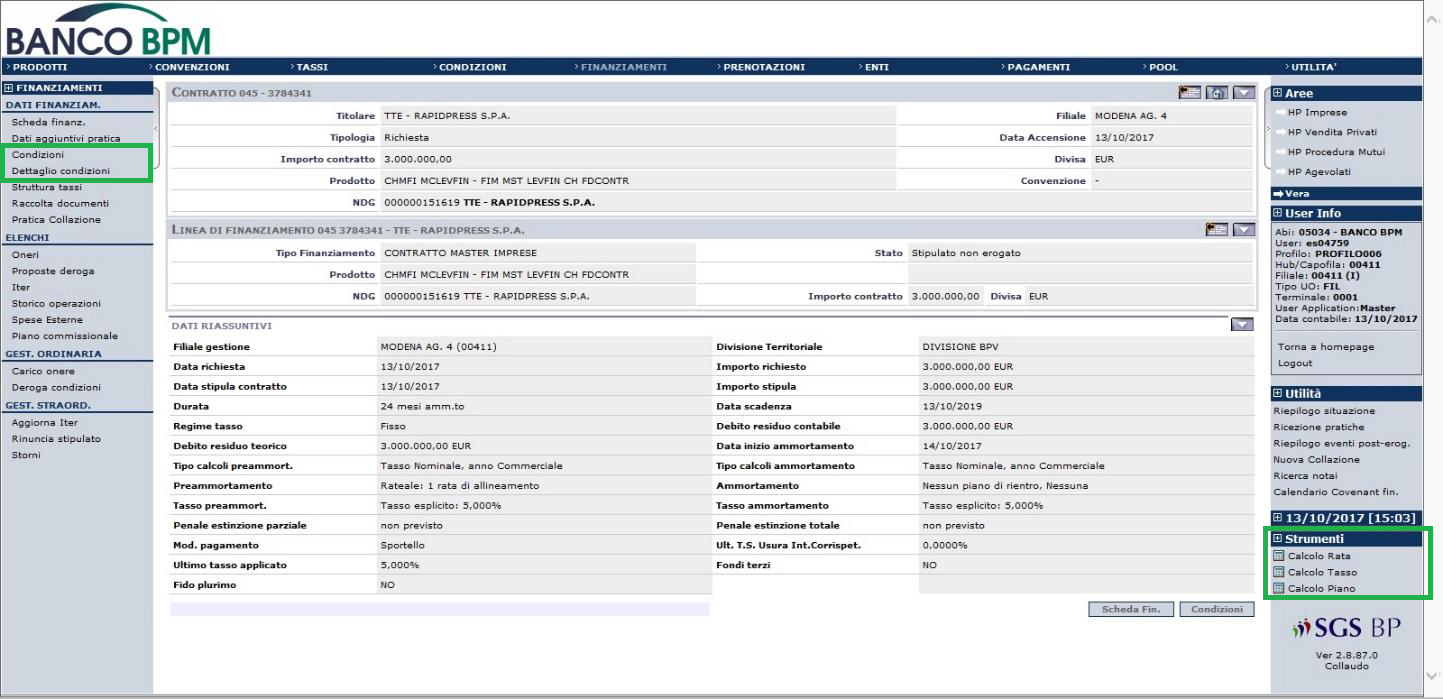
\includegraphics[width=0.95\textwidth]{immagini/Elise_postCMU}
	   	\caption{Posizionamento possibile integrazione calcolo CMU in ELISE -\\ Fonte immagine originale: documento di collaudo interno aziendale}
	\end{figure}
	
	
	Integrando il mio operato più a basso livello all'interno dell'architettura, invece, l'utente utilizzatore di ELISE avrà la possibilità di ottenere automaticamente il risultato del calcolo della Commissione di Mancato Utilizzo soltando delimitando un \textit{range} temporale su cui operare. Migliore sarebbe l'opzione che prevede che l'utente scelga tale \textit{range} da un menu a tendina ed in base a questo effettuare il calcolo; questa variante a mio avviso è migliore perché nella pratica questa commissione viene solitamente calcolata su scaglioni trimestrali, difficilmente a scaglioni temporali di minore durata.\\
	
	Conseguentemente a questo inoltre, una volta calcolata la CMU l'utente utilizzatore di ELISE potrà trovare tale commissione, sotto forma di onere, addizionata all'importo della prossima rata da pagare.\\
	
	Avendo a disposizione questa funzionalità gli utenti degli istituti di credito che utilizzano ELISE non dovranno più calcolare manualmente questo tipo di commissione e aggiungerla manualmente come onere alle rate ma sarà fatto tutto da un procedimento automatico, innescabile semplicemente impostando tale tipo di \textit{feature} alla tipologia di "\textit{Prodotto di Finanziamento}" [\ref{ELISE}]. Tale proprietà potrà essere impostata dal menu di spalla laterale sinistra in ELISE, come evidenziato dalla figura precedente.             % Stage
%% !TEX encoding = UTF-8
% !TEX TS-program = pdflatex
% !TEX root = ../tesi.tex
% !TEX spellcheck = it-IT

%**************************************************************
\chapter{Valutazione retrospettiva}
\label{cap:valutazione-retrospettiva}
%**************************************************************

%\intro{Breve introduzione al capitolo}\\

%**************************************************************
\section{Conoscenze preliminari}

Per lo svolgimento del lavoro di stage non era richiesta una conoscenza approfondita dei linguaggi che si andavano ad utilizzare, proprio perché era prevista una prima fase di studio delle tecnologie e lo scopo dello stage era formativo, in modo da arricchire le mie competenze curricolari.\\

Nonostante ciò, la mia preparazione riguardo le tecnologie web,	maturata nel corso di studi, è stata molto utile nel comprendere i nuovi aspetti che andavo a trattare in azienda, consolidando tali conoscenze. L'aspetto che ha richiesto maggiore impegno da parte mia è stata l'analisi del progetto ELISE e le prime fasi di approccio ad esso, nel tentativo di individuare percorsi a me conosciuti e comprendere al meglio i suoi funzionamenti, essendo un applicativo molto grande ed intricato nei suoi processi.\\

Il Corso di Laurea triennale in Informatica mi ha fornito una buona formazione nello sviluppo software, permettendomi la comprensione del ciclo di sviluppo applicato al progetto richiesto nel mio periodo di stage, senza troppe difficoltà.\\
	
Questi aspetti preliminari hanno permesso che il progetto di stage non subisse imprevisti o interruzioni dovute a mie lacune, concentrandomi per più tempo sugli studi e le applicazioni previste dal piano di lavoro.

%**************************************************************
\newpage
\section{Obiettivi raggiunti}

Durante il lavoro di stage ho svolto le attività necessarie al raggiungimento degli obiettivi prefissati in fase di pianificazione.
Le seguenti tabelle raccolgono i risultati ottenuti per ciascun obbiettivo, suddividendoli per la loro categoria.

\subsubsection{Obbligatori}

	\begin{table}[H]
		\def\arraystretch{1.2}
		\begin{tabular}{ | p{10cm} | p{2cm} | }
		
		\rowcolor{Gray}
		\hline \textbf{Obiettivo} & \textbf{Esito} \\ \hline
		
		Studio e acquisizione di padronanza dell'ambiente di sviluppo Eclipse & Completato \\ \hline
		Studio e comprensione della piattaforma Java EE & Completato \\ \hline
		Installazione e utilizzo di diversi \textit{application server} e diverse JVM & Completato \\ \hline
		Acquisizione familiarità con la programmazione web in ambito Java (tecnologie JSP, JSTL, Servlet\glossario ) & Completato \\ \hline
		Acquisizione tecniche di programmazione con framework Struts & Completato \\ \hline
		Studio e utilizzo del sistema di versionamento RTC & Completato \\ \hline
		Studio e utilizzo della tecnologia AJAX\glossario & Completato \\ \hline
		Implementazione di applicazioni di esempio per le funzionalità basilari & Completato \\ \hline
		Analisi di una complessa applicazione reale in architettura Java EE & Completato \\ \hline
		Integrazione nel team di sviluppo e acquisizione competenze nelle dinamiche di gruppo & Completato \\ \hline
		Comprensione e acquisizione familiarità con la documentazione di analisi e specifica delle attività & Completato \\ \hline
		Implementazione di modifiche basilari dell'applicazione ambito di progetto & Completato \\ \hline
		Implementazione di modifiche complesse dell'applicazione ambito di progetto & Completato \\ \hline
		
		\end{tabular}
		\vspace{1mm}
		\caption{Tabella degli obiettivi obbligatori raggiunti durante il lavoro di stage}
	\end{table}


\subsubsection{Desiderabili}

	\begin{table}[H]
		\def\arraystretch{1.2}
		\begin{tabular}{ | p{10cm} | p{2cm} | }
		
		\rowcolor{Gray}
		\hline \textbf{Obiettivo} & \textbf{Esito} \\ \hline
		
		Raggiungimento di un buon livello di autonomia nell'utilizzo di Java EE & Completato \\ \hline
		Raggiungimento di un buon livello di autonomia nell'utilizzo di tecnologie web standard (HTML, CSS, JavaScript) & Completato \\ \hline
		Raggiungimento di un buon livello di autonomia nell'utilizzo di tecnologie web in ambito Java (JSP, JSTL, Servlet\glossario ) & Completato \\ \hline
		Acquisizione tecniche di programmazione con framework alternativi (Maven e Hibernate) & Completato \\ \hline
		Studio e utilizzo di un sistema di versionamento alternativo (SVN) & Completato \\ \hline
		Studio e utilizzo della libreria per le stampe PDF, iText & Completato \\ \hline
		Studio e utilizzo della libreria per il \textit{logging}, Log4J & Completato \\ \hline
		Capacità di portare a termine le attività lavorative secondo le tempistiche stabilite, anche in situazioni critiche & Completato \\ \hline
		Conoscenza delle norme di sicurezza relative all'ambiente di lavoro & Completato \\ \hline
		
		\end{tabular}
		\vspace{1mm}
		\caption{Tabella degli obiettivi desiderabili raggiunti durante il lavoro di stage}
	\end{table}


\subsubsection{Facoltativi}

	\begin{table}[H]
		\def\arraystretch{1.2}
		\begin{tabular}{ | p{10cm} | p{2cm} | }
		
		\rowcolor{Gray}
		\hline \textbf{Obiettivo} & \textbf{Esito} \\ \hline
		
		Studio delle meccaniche di comunicazione con l'area di business per la gestione dei dati & Completato \\ \hline
		Partecipazione alle attività di test di integrazione dell'applicazione ambito di progetto & Non \newline completato \\ \hline
		Partecipazione alle attività di collaudo dell'applicazione ambito di progetto & Completato \\ \hline
		Rilascio delle nuove funzionalità sviluppate nelle attività assegnate & Completato \\ \hline
		
		\end{tabular}
		\vspace{1mm}
		\caption{Tabella degli obiettivi facoltativi raggiunti durante il lavoro di stage}
	\end{table}

Si denota quindi un completamento globale degli obiettivi pianificati, ad unica eccezione delle attività di integrazione software, in quanto queste sono state assegnate ad altri team di sviluppo.
%Durante il mio lavoro infatti si succedevano molteplici dinamismi all'interno dell'azienda e io e il tutor non abbiamo potuto far fronte a tutti. \\

%**************************************************************
\newpage
\section{Bilancio formativo}

A partire dalle mie conoscenze preliminari nell'ambito ricoperto dal progetto ho avuto modo, tramite il lavoro di stage, di ampliare le mie conoscenze e spingermi verso concetti a me nuovi riguardo la progettazione architetturale nel web. Grazie alle spiegazioni del tutor aziendale, a cui devo la facilità con cui si è svolto il progetto, ho potuto ricevere molte nozioni, anche non approfondite ma che di volta in volta mi abilitavano a nuove possibilità di implementazione, inglobandomi in un ambiente stimolante e dinamico.\\

Tutto ciò mi ha permesso di imparare molto, arricchendo le mie conoscenze nello sviluppo web, utilizzando software di cui non ero pratico e consolidando le mie conoscenze a livello teorico, applicandole nella realtà.\\

Ho guadagnato padronanza degli sviluppi web mediante Java EE e le tecnologie incluse in tale piattaforma, come JSP e JSTL che non avevo mai utilizzato. Ho interagito con sistemi diversi di versionamento, ho imparato nuove tecniche di programmazione, come AJAX\glossario , la Reflection\glossario\ e le \textit{properties}, di cui non ero a conoscenza o avevo ricevuto solo alcuni accenni all'Università. Ho anche ottenuto una buona padronanza con un nuovo ambiente di sviluppo e diverse librerie molto utili, ad esempio per il \textit{logging}.\\

Grazie allo stage in Sopra Steria ho avuto modo di crescere professionalmente e vivere personalmente un'esperienza lavorativa che ha avuto luogo in un ambiente molto dinamico e stimolante. Ho interagito con molti colleghi anche in altre sedi e ho avuto una visione generale dei processi di un'azienda rilevante nel settore ICT\glossario .\\

Presumibilmente il Corso di Laurea triennale in Informatica è ancora in fase di rodaggio, dopo il passaggio a semestri, si è sentita la pesantezza del carico distribuito	male nei vari insegnamenti, specie riguardo le propedeuticità che spesso in questo corso rappresentano uno scoglio per gli studenti.\\

Ho apprezzato che il corso di Ingegneria del Software abbia dato luogo a diversi seminari tecnoloici e abbia incentrato i progetti presentati nell'uso di moderni linguaggi e paradigmi di programmazione, al contrario degli altri corsi che rimangono piuttosto canonici e trattano poche innovazioni negli ambiti di studio.

% Conclusioni
\newpage
Oltre al successo nel soddisfare gli obiettivi prefissati per la valutazione positiva dello stage, a livello personale ho avuto molta soddisfazione nel raggiungere anche gli obiettivi	personali che mi ero posto nella ricerca dello stage.\\

Ho lavorato in un ambiente professionale e collaborativo, applicando le mie competenze per scopi pratici e utili al team di sviluppo. Ho avuto modo di arricchire il mio profilo tecnico e lavorativo diventando un potenziale interesse ancora maggiore verso le aziende ICT\glossario , come la stessa Sopra Steria che mi ha ospitato.\\

	Sono rimasto soddisfatto quindi dell'esperienza fatta, ma anche della formazione guadagnata presso l'Università nel Corso di Laurea triennale in informatica, stabilendo una solida base di studi su cui costruire la mia carriera.\\
	
	Mi è stata data la possibilità di proseguire il mio percorso di stage in vista di una futura assunzione, dopo il conseguimento di un totale di sei mesi di tirocinio, compresi i due appena svolti. Pertanto ho intenzione di procedere in tale direzione, vista anche la soddisfazione da ambo le parti dopo questa esperienza.

	
%\gls{ajax}
%
%\gls{cics}
%
%\gls{cobol}
%
%\gls{covenant}
%
%\gls{ctg}
% 
%\gls{dbms}
%\gls{eis}
%
%\gls{front-end}
%
%\gls{iframe}
%
%\gls{ict}
%
%\gls{jar}
%
%\gls{javabeans}
%
%\gls{jca}
%
%\gls{jdbc}
%
%\gls{jndi}
%
%\gls{mvc}
%
%\gls{reflection}
%
%\gls{servlet}


%**************************************************************
%\section{Conclusioni}
%Valutazione retrospettiva dell'esperienza di stage.
             % Valutazioni

%**************************************************************
% Materiale finale
%**************************************************************
\appendix 
%aggiunto per fix glossario                              
\glsaddall
\printglossaries
\backmatter
%% !TEX encoding = UTF-8
% !TEX TS-program = pdflatex
% !TEX root = ../Lahmer_Abdelilah_tesi.tex
% !TEX spellcheck = it-IT

%**************************************************************
% Ringraziamenti
%**************************************************************
\cleardoublepage
\phantomsection
\pdfbookmark{Ringraziamenti}{ringraziamenti}

\leavevmode	\newline

\begin{flushright}{
	\slshape    
	``He who does not thank people, does not thank God''} \\ 
	\medskip
    --- Prophet Muhammad (PBUH)
\end{flushright}


\bigskip

\begingroup
\let\clearpage\relax
\let\cleardoublepage\relax
\let\cleardoublepage\relax

\chapter*{Ringraziamenti}

 \noindent \textit{Innanzitutto vorrei ringraziare i miei genitori, Najeh e Latifa, per avermi accompagnato e concesso di arrivare fin qui. Grazie inoltre alla mia intera famiglia per il sostegno e per essermi sempre stati vicini.}\\

\noindent \textit{Ringrazio i compagni di studi per tutti i bellissimi anni passati insieme, in particolare i colleghi di Answer Group.}\\

\noindent \textit{La più sentita gratitudine inoltre agli amici più stretti, in particolare ringrazio Hamza, Abdourahmane, Amir, Mustafa e Sara per tutto il loro affetto e sostegno ricevuto.}\\

%\noindent \textit{Ringrazio Sopra Steria Group S.p.A. e tutti i dipendenti della sede di Padova per avermi accolto e seguito durante il tirocinio.}\\

\noindent \textit{Ringrazio sentitamente, infine, il prof. \myProf, relatore della mia Tesi, per l'aiuto, i preziosi consigli e la pazienza che mi ha dedicato per lo svolgimento del lavoro.}\\

\bigskip

\noindent\textit{\myLocation, \myTime}
\hfill \myName

\endgroup

%\blankpage
%\blankpage


\end{document}

$
The book class has some advantages over the report class since it defines three
commands (\frontmatter, \mainmatter, and \backmatter) that control the page
number and chapter numbering formats. In the frontmatter, pages are numbered
with lower case Roman numbers (i, ii, iii, etc.) and the chapters are not numbered
(as if the asterisk version /chapter*{} was used). In the mainmatter, pages are
numbered with Arabic numbers (the numbers start from 1) and the chapters
are numbered with Arabic numbers as well. In the backmatter, the pages are
numbered as in the mainmatter (numbering continues) but the chapters are not
numbered.
$
